\section{Supplementary material}
\label{sec:supplementary_material}

\subsection{SNP calling thresholds}
\label{sec:SNP_calling_thresholds}
Genotype calling can incur in two types of error, namely a heterozygote wrongly identified as homozigote ($HET \rightarrow HOM$) and the reverse case ($HOM \rightarrow HET$). 
Under the simplifying hypothesis of absence of sequencing errors and homogeneous sequencing quality, it is possible to estimate error rates for a tetraploid genome using the following formula:

\begin{equation}
\begin{cases}
0.75^{N_h} + 0.25^{N_h} & HET_{3-1} \rightarrow HOM \\ 
2 \times 0.5^{N_h}      & HET_{2-2} \rightarrow HOM \\ 
0                       & HOM \rightarrow HET
\end{cases}
\end{equation}

Where $N_h$ is the minimum number of reads required to label a stack of aligning reads as heterozygote. The discussed case of $N_h = 11$ brings to a total expected $HET \rightarrow HOM$ error rate of 4.22\%.\\
The hypothesis mentioned above greatly simplyfies the real case (e.g. $HOM \rightarrow HET$ errors can not happen, since a homozigote will always produce 100\% of reads of the same type). When accounting sequencing errors and reads quality a term for $HOM \rightarrow HET$ appears, due to reads sequenced as the wrong allele. In the presented study we thus applied a threshold of 4 required reads per stack to call a homozigote to minimize this kind of error.

\subsection{Supplementary figures}
\label{sec:supplementary_figures}

\begin{figure}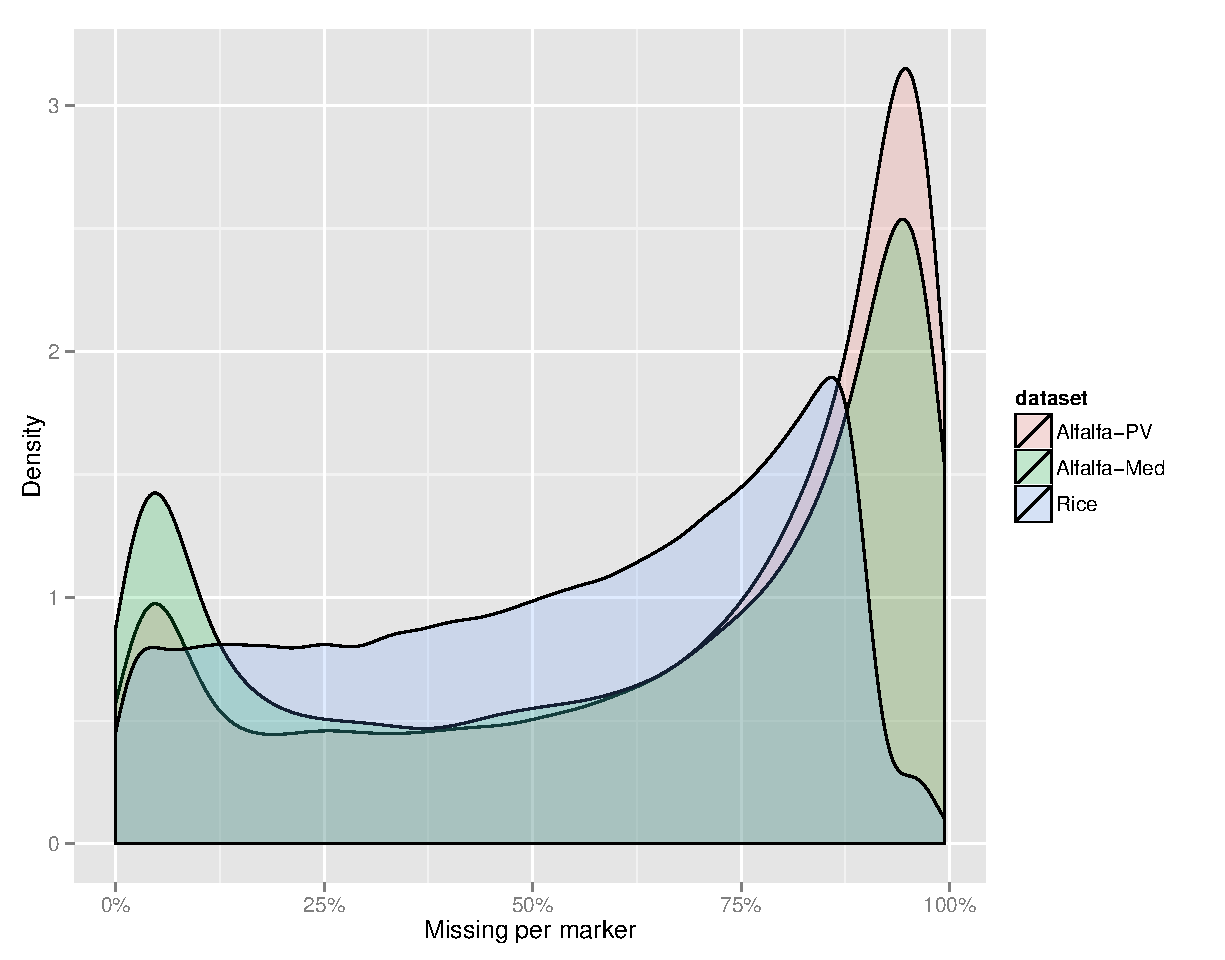
\includegraphics[width=0.95\textwidth]{SupplFig01_miss_per_marker.pdf}
\caption{Distribution of missings-per-marker rates in the three datasets. This is a
density plot, so all curves delimit the same unitary area.}
\end{figure}

\begin{figure}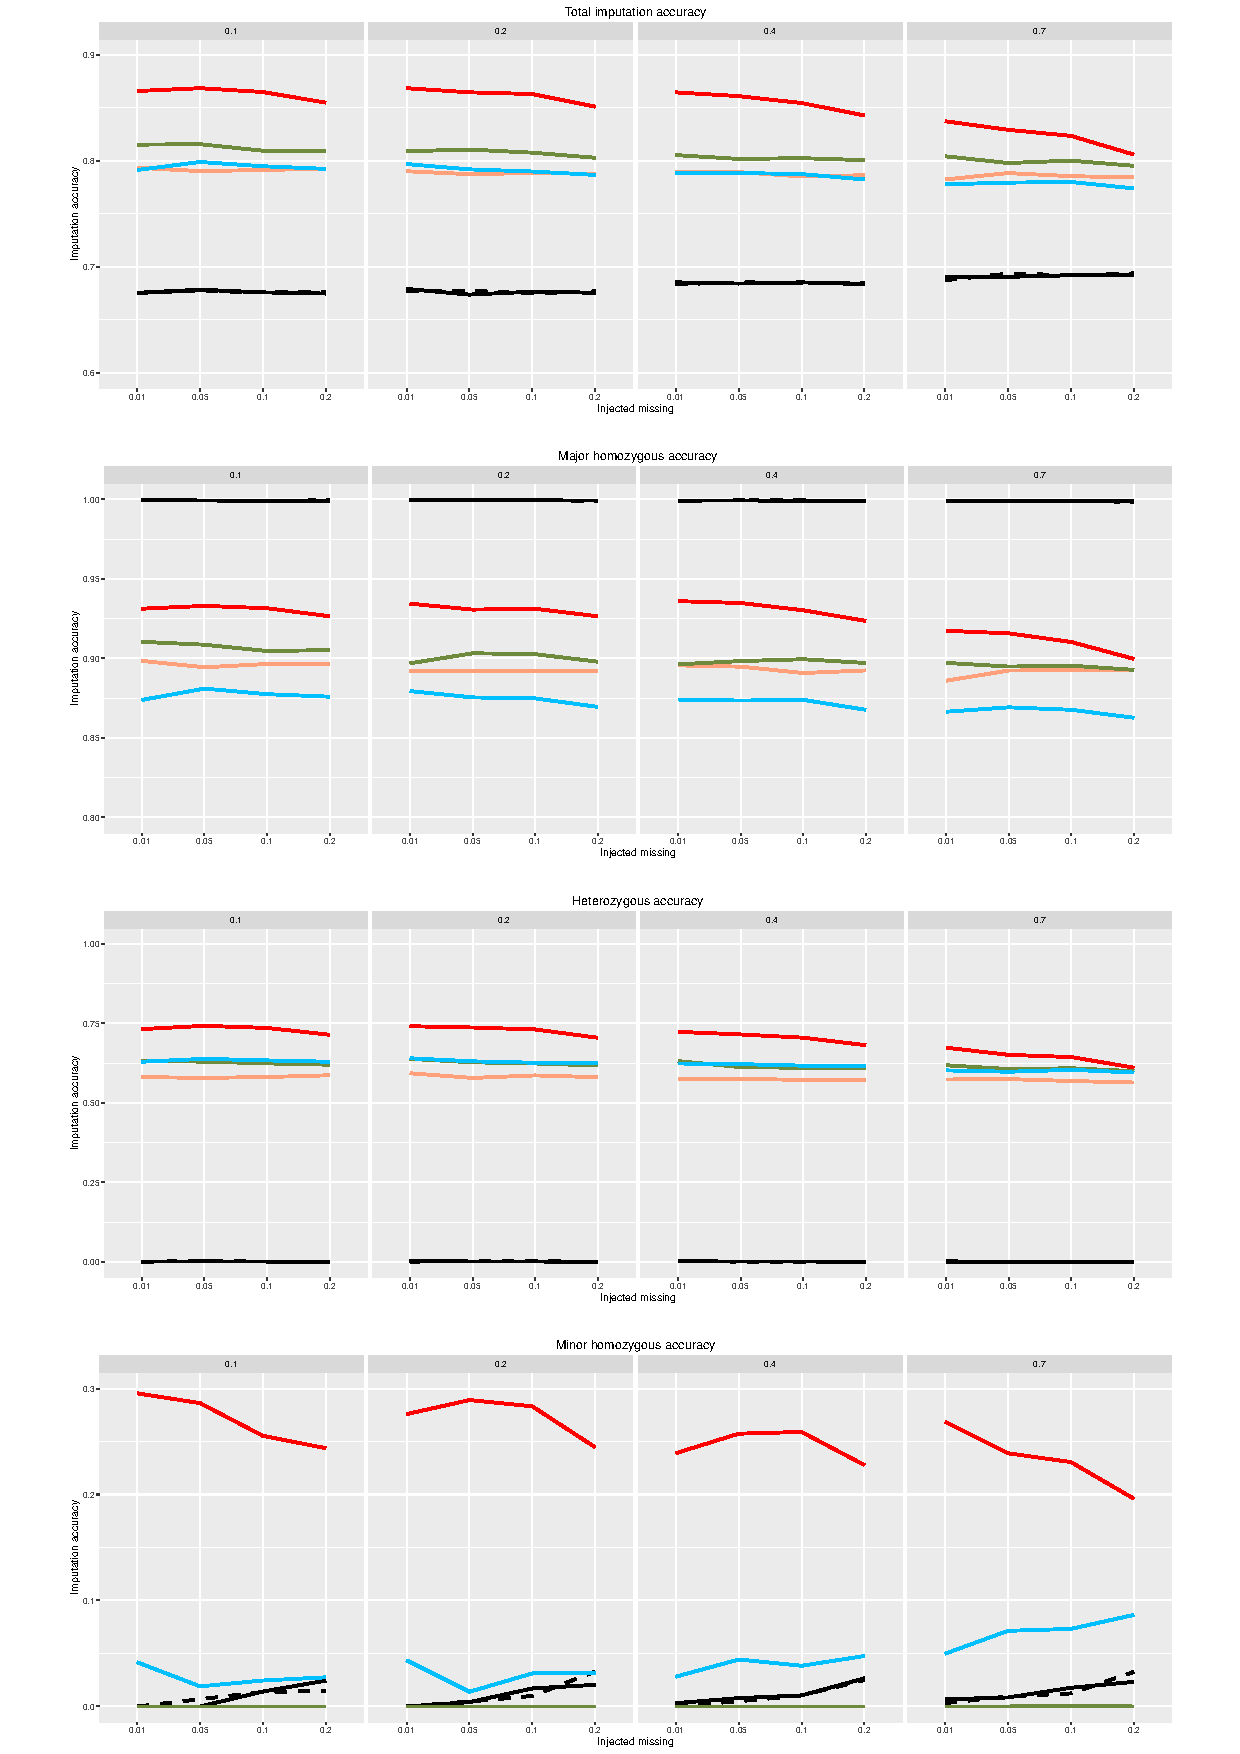
\includegraphics[width=0.95\textwidth]{figure_reforma.pdf}\caption{
imputation accuracies overall, for the major homozygous genotype (AA), for heterozygotes (AB), and for the minor homozygous genotype (BB) in datasets consisting of
10\%, 20\%, 40\% and 70\% allowed missing data per locus (boxes) with 1\%, 5\%, 10\% and 20\%
additional missing values artificially introduced (x-axis) for alfalfa population Alfalfa-Med.
Lines colors represent the five imputation algorithms: MNI (salmon), KNNI (red), SVDI (blue), RFI (green), Beagle with ordered markers (solid black) and Beagle with unordered markers (dashed black)}\end{figure}

\begin{figure}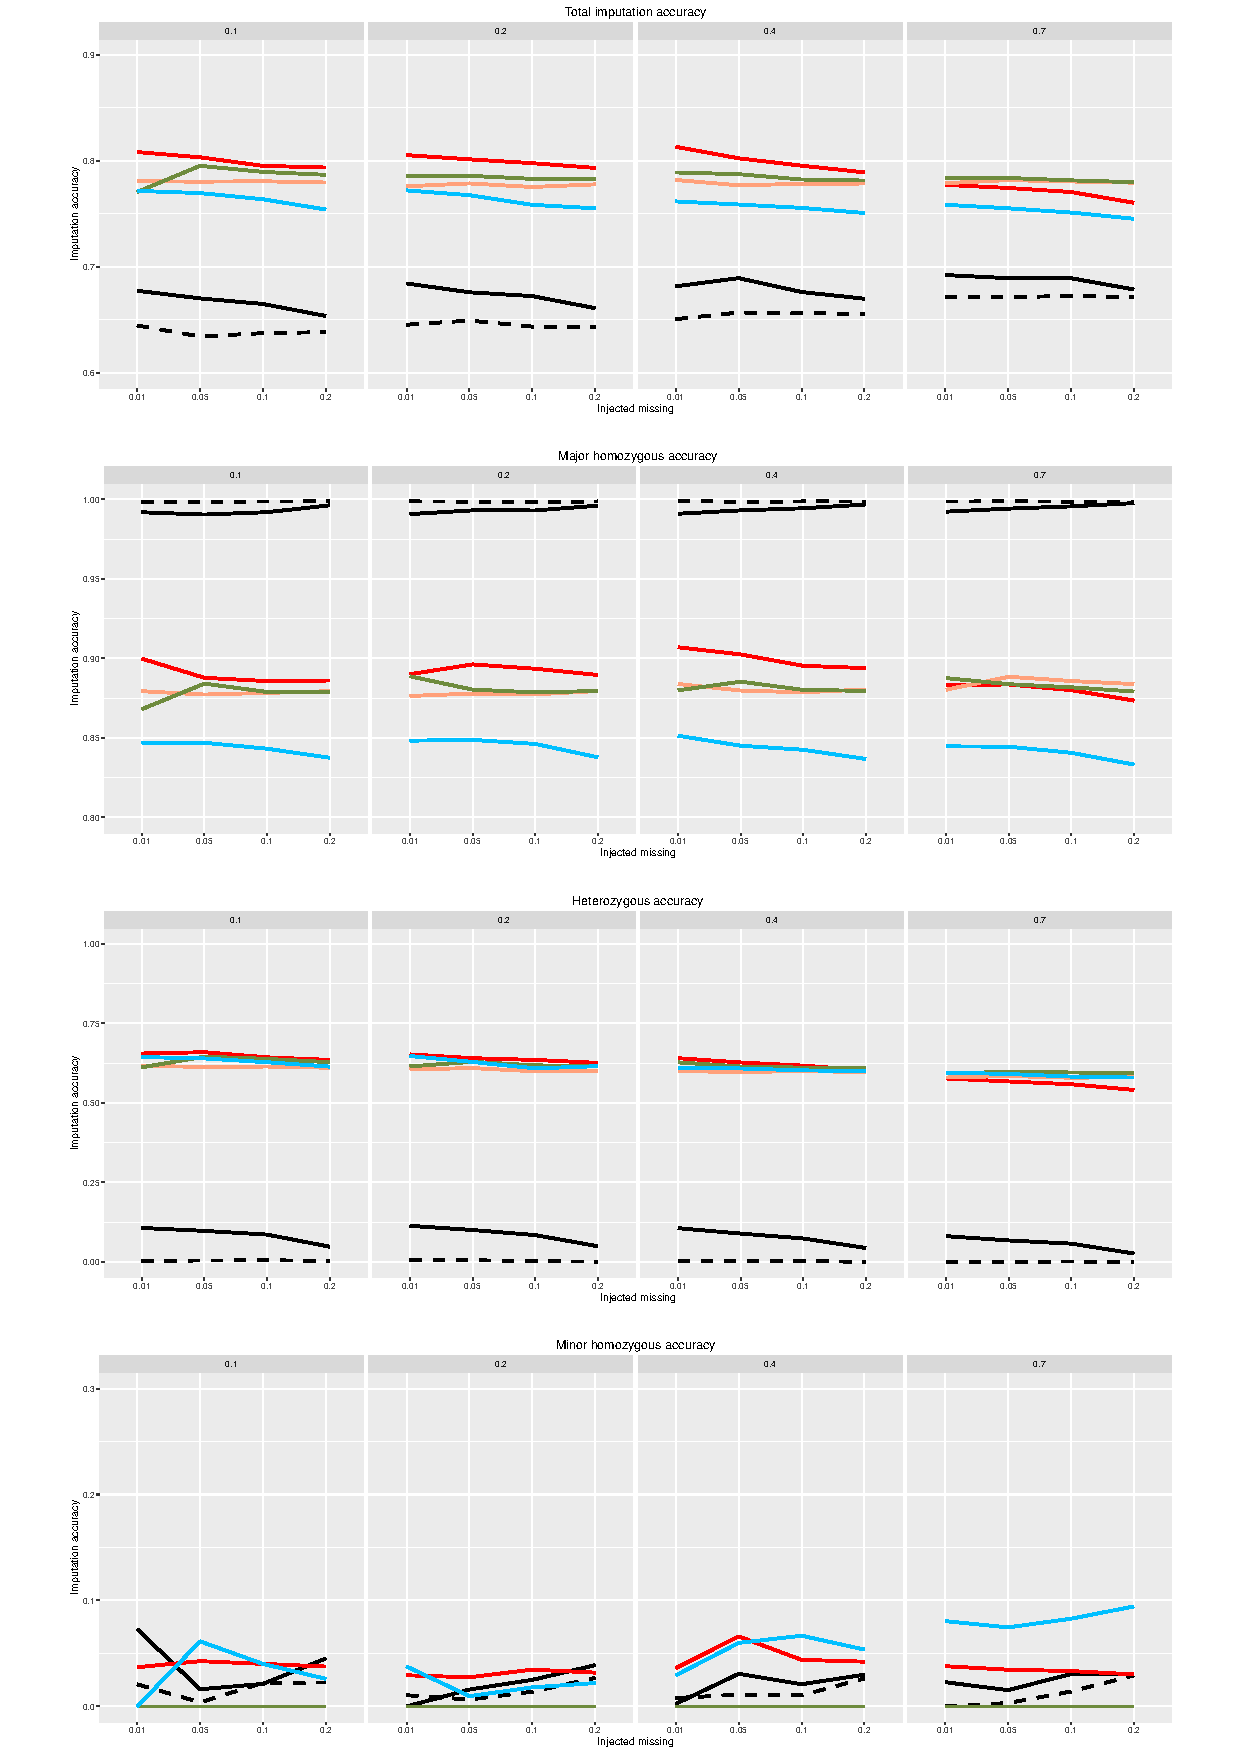
\includegraphics[width=0.95\textwidth]{figure_lodi.pdf}\caption{
imputation accuracies overall, for the major homozygous genotype (AA), for heterozygotes (AB), and for the minor homozygous genotype (BB) in datasets consisting of
10\%, 20\%, 40\% and 70\% allowed missing data per locus (boxes) with 1\%, 5\%, 10\% and 20\%
additional missing values artificially introduced (x-axis) for alfalfa population Alfalfa-PV.
Lines colors represent the five imputation algorithms: MNI (salmon), KNNI (red), SVDI (blue), RFI (green), Beagle with ordered markers (solid black) and Beagle with unordered markers (dashed black)}\end{figure}

\begin{figure}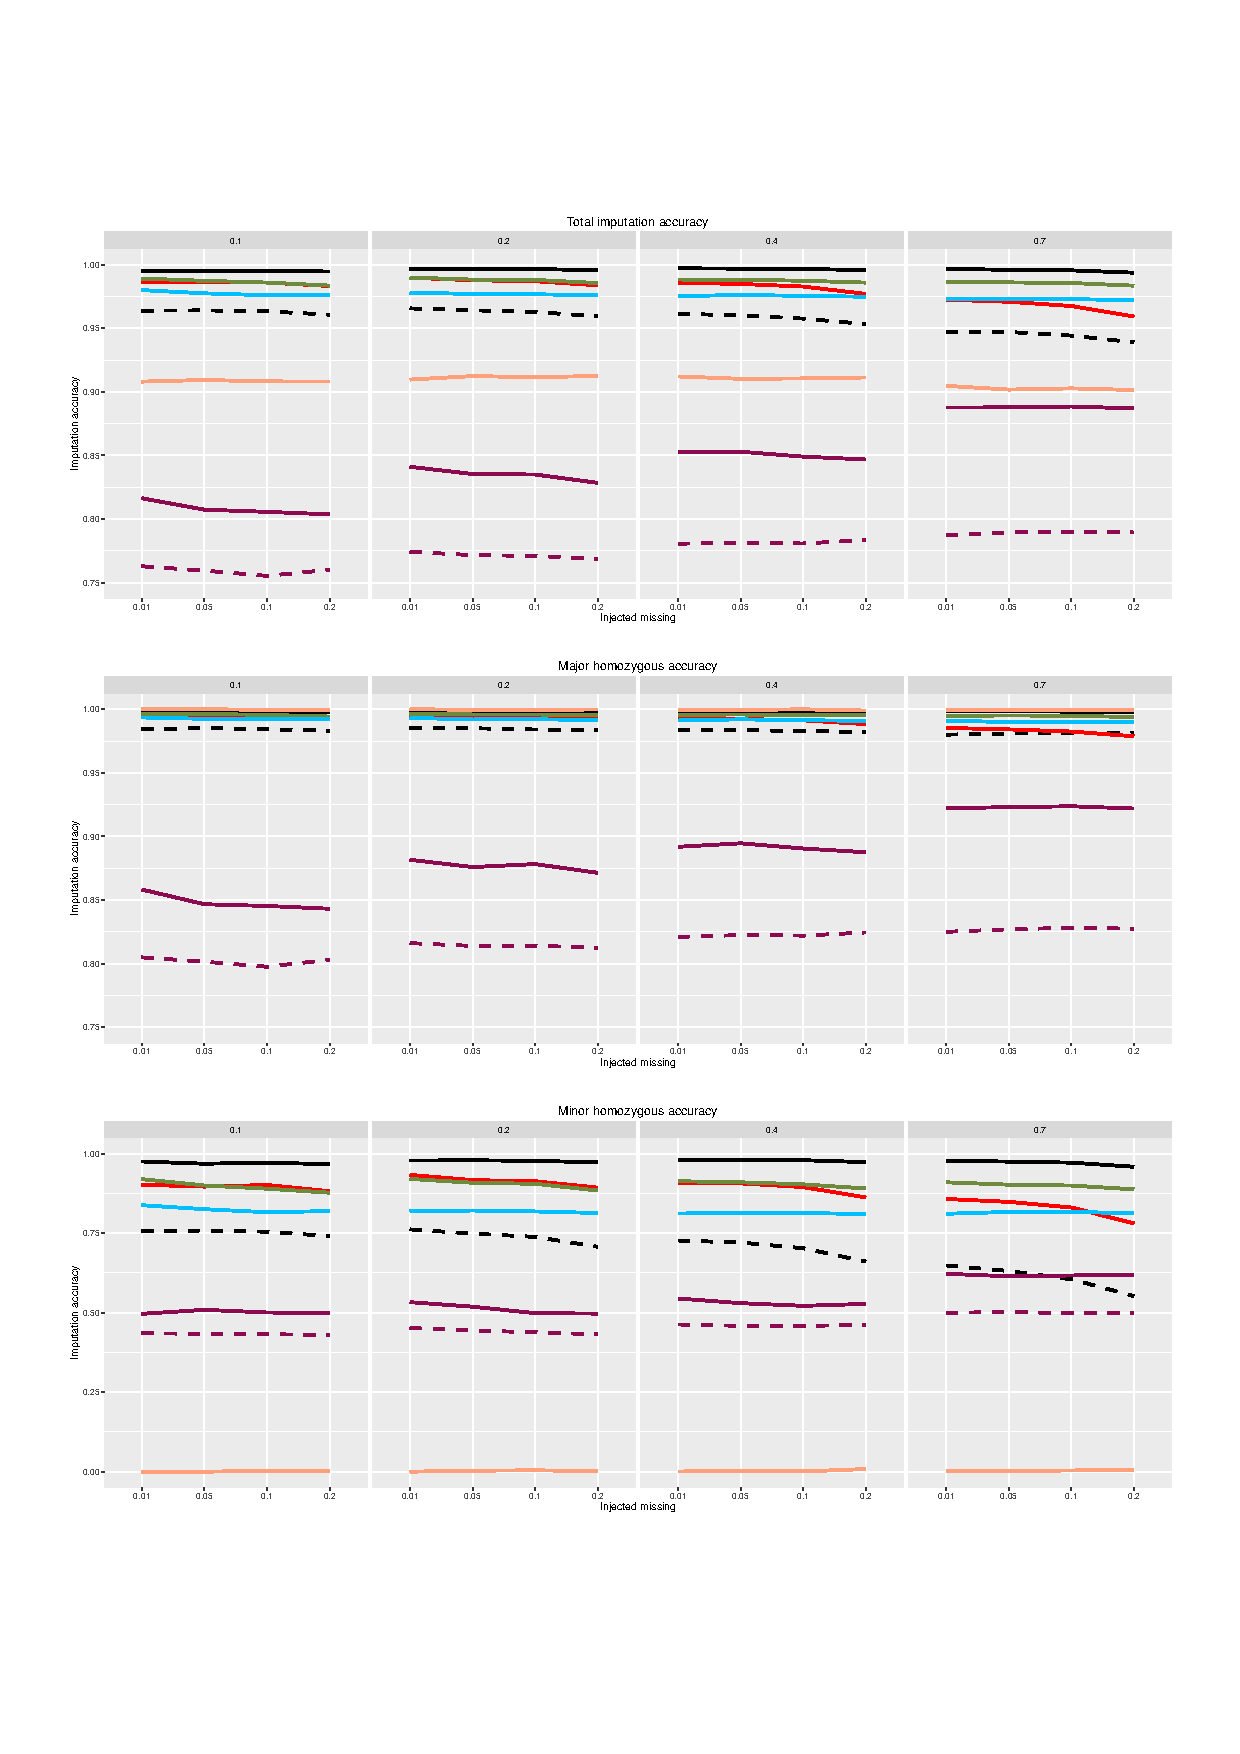
\includegraphics[width=0.95\textwidth]{figure_rice_chrom_1.pdf}\caption{
imputation accuracies overall, for the major homozygous genotype (AA) and for the minor homozygous genotype (BB) in datasets consisting of
10\%, 20\%, 40\% and 70\% allowed missing data per locus (boxes) with 1\%, 5\%, 10\% and 20\%
additional missing values artificially introduced (x-axis) for rice chromosome 1 data.
Lines colors represent the five imputation algorithms: MNI (salmon), KNNI (red), SVDI (blue), RFI (green), Beagle with ordered markers (solid black) and Beagle with unordered markers (dashed black)}\end{figure}

\begin{figure}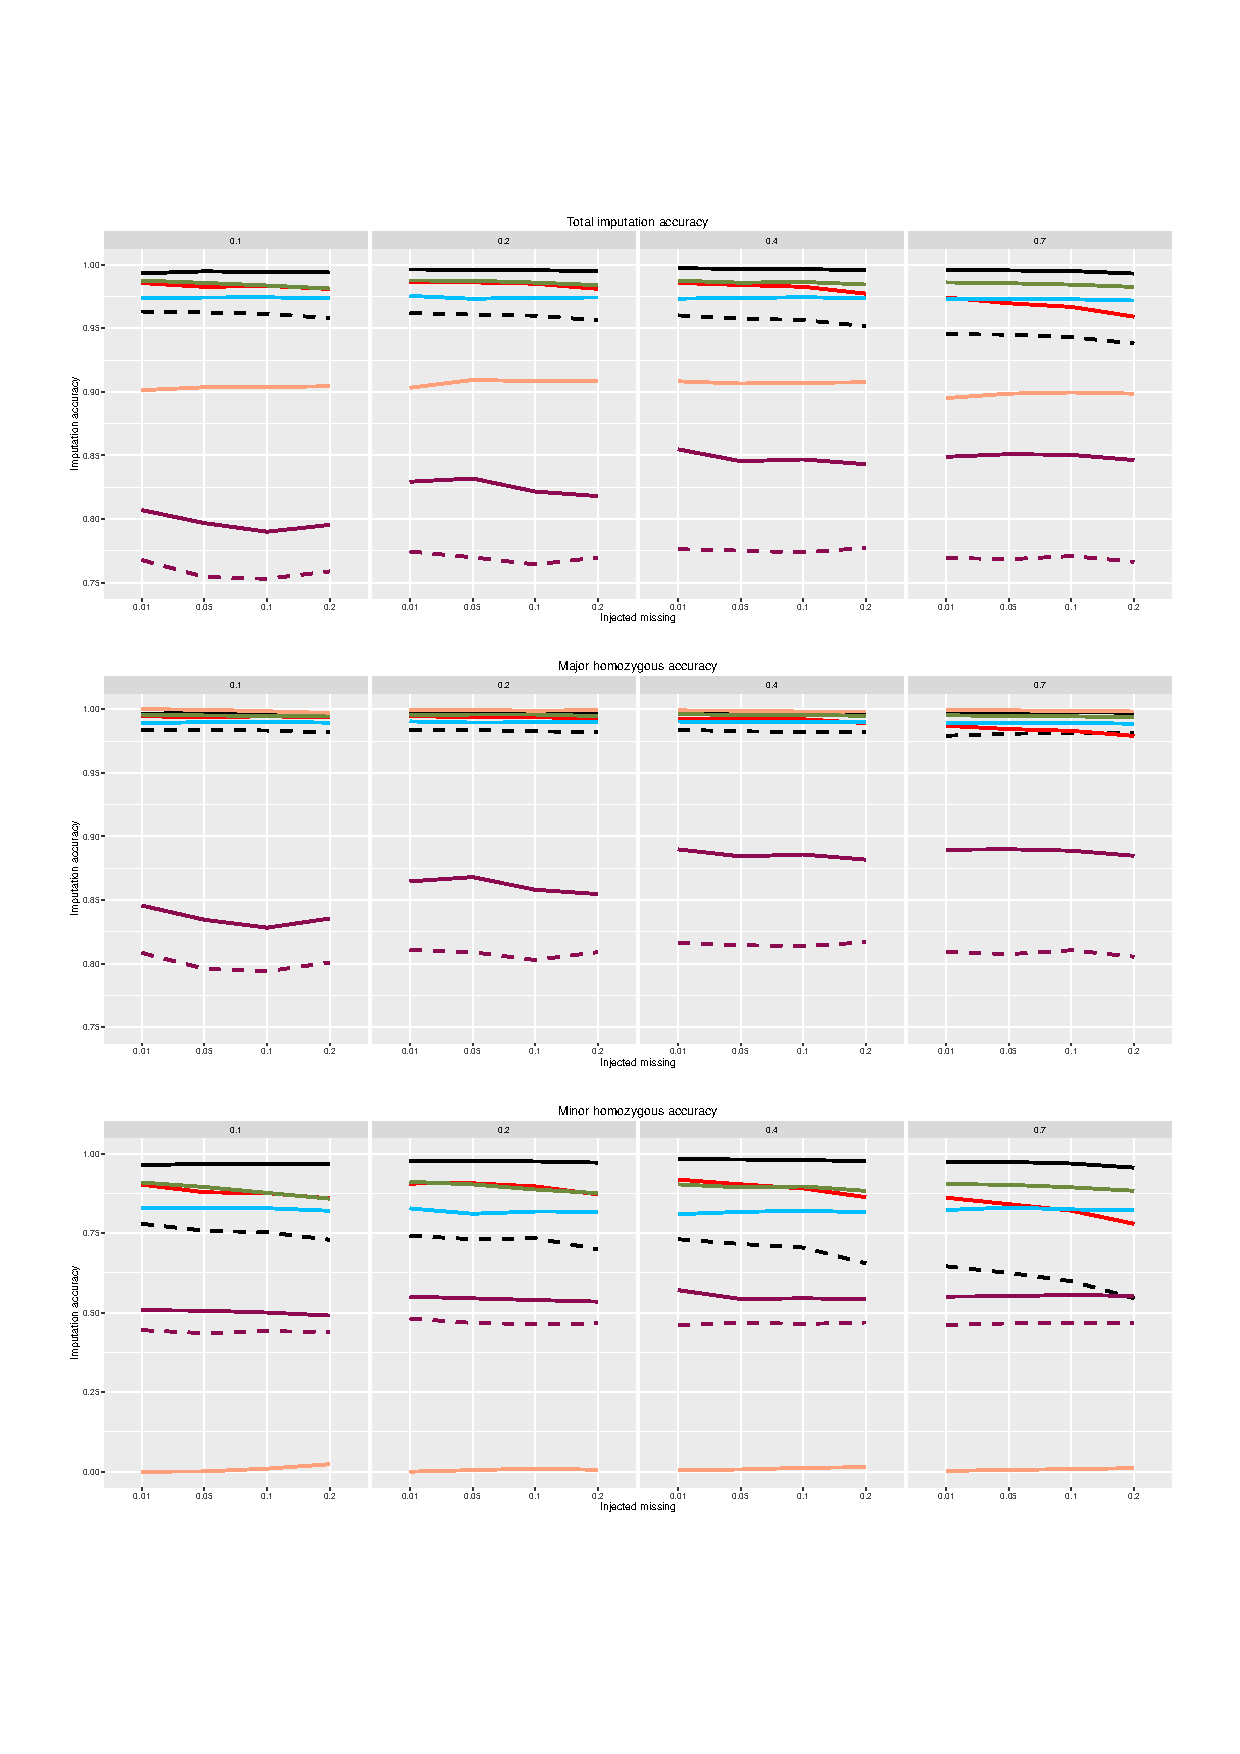
\includegraphics[width=0.95\textwidth]{figure_rice_chrom_2.pdf}\caption{
imputation accuracies overall, for the major homozygous genotype (AA) and for the minor homozygous genotype (BB) in datasets consisting of
10\%, 20\%, 40\% and 70\% allowed missing data per locus (boxes) with 1\%, 5\%, 10\% and 20\%
additional missing values artificially introduced (x-axis) for rice chromosome 2 data.
Lines colors represent the five imputation algorithms: MNI (salmon), KNNI (red), SVDI (blue), RFI (green), Beagle with ordered markers (solid black) and Beagle with unordered markers (dashed black)}\end{figure}

\begin{figure}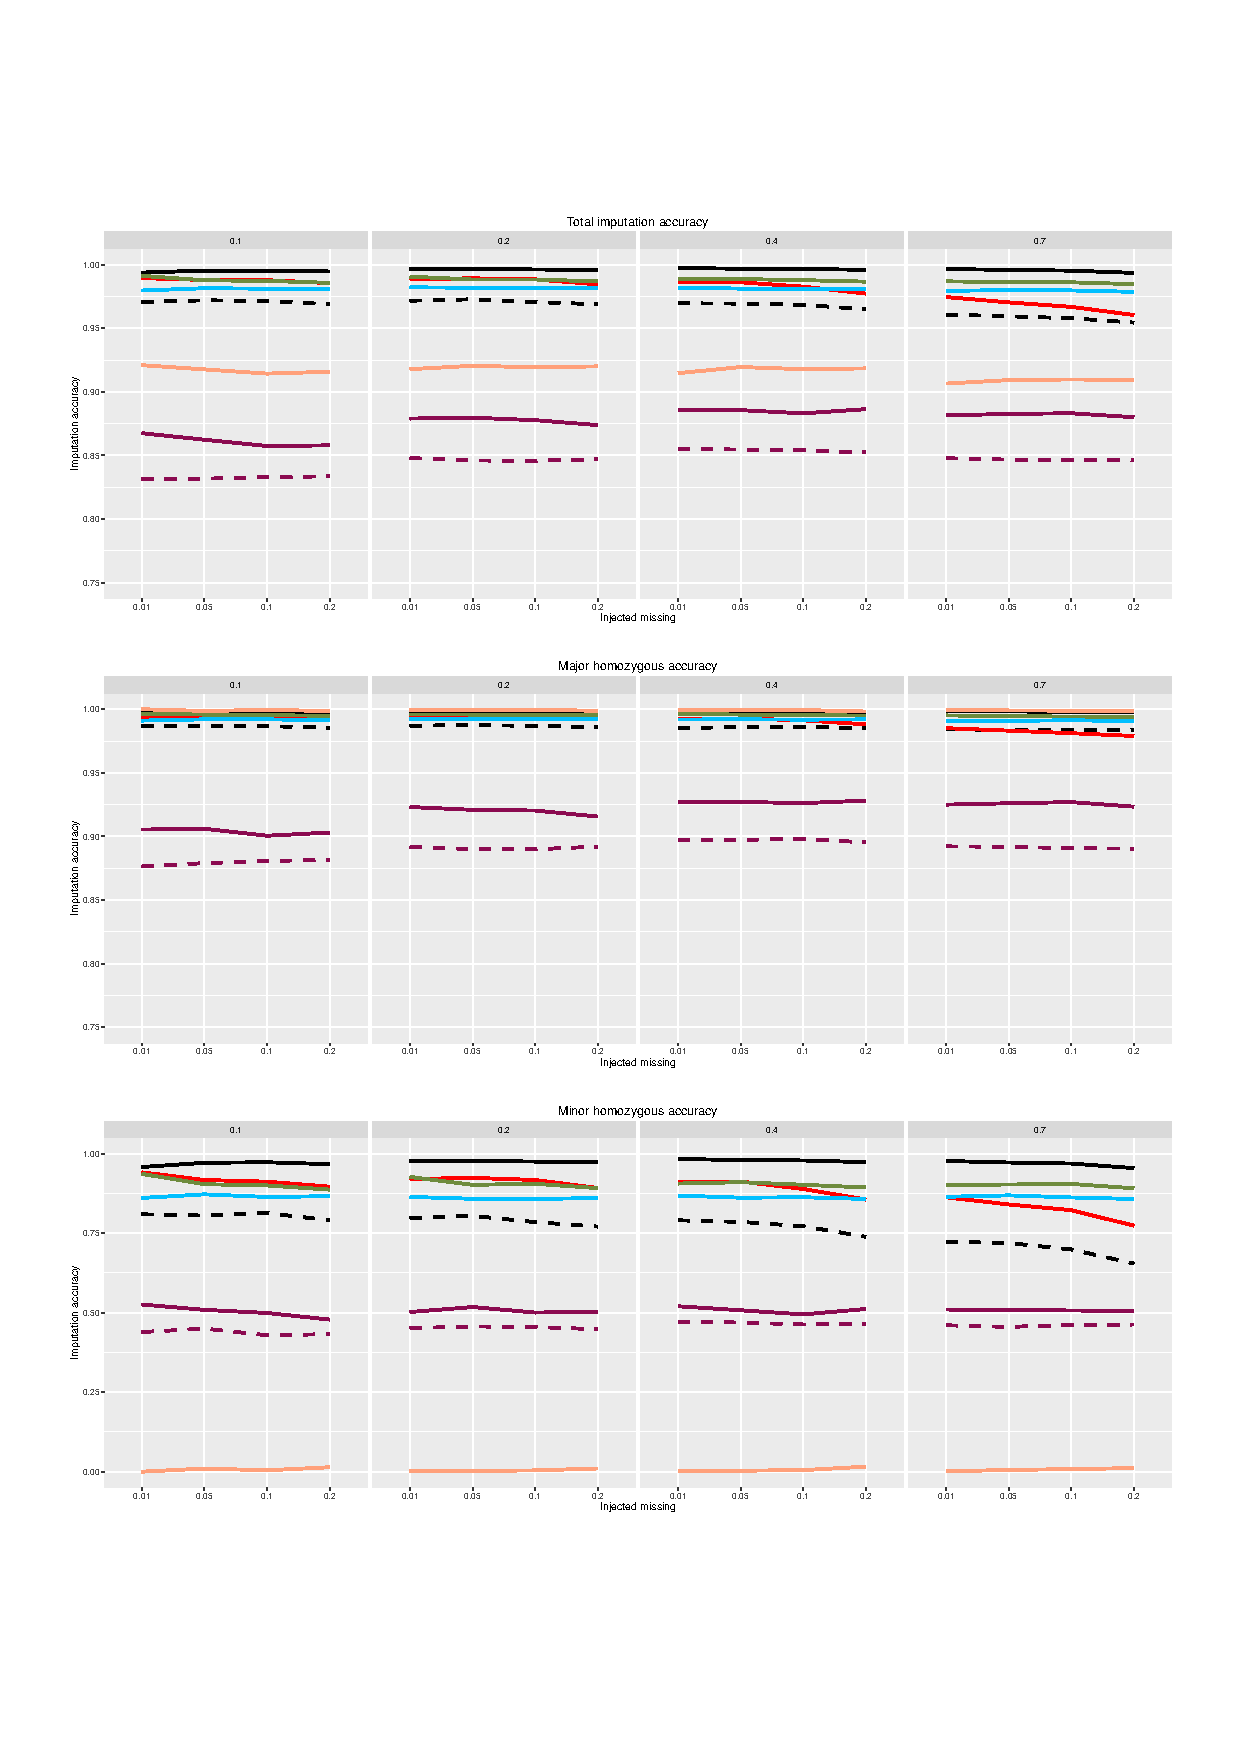
\includegraphics[width=0.95\textwidth]{figure_rice_chrom_3.pdf}\caption{
imputation accuracies overall, for the major homozygous genotype (AA) and for the minor homozygous genotype (BB) in datasets consisting of
10\%, 20\%, 40\% and 70\% allowed missing data per locus (boxes) with 1\%, 5\%, 10\% and 20\%
additional missing values artificially introduced (x-axis) for rice chromosome 3 data.
Lines colors represent the five imputation algorithms: MNI (salmon), KNNI (red), SVDI (blue), RFI (green), Beagle with ordered markers (solid black) and Beagle with unordered markers (dashed black)}\end{figure}

\begin{figure}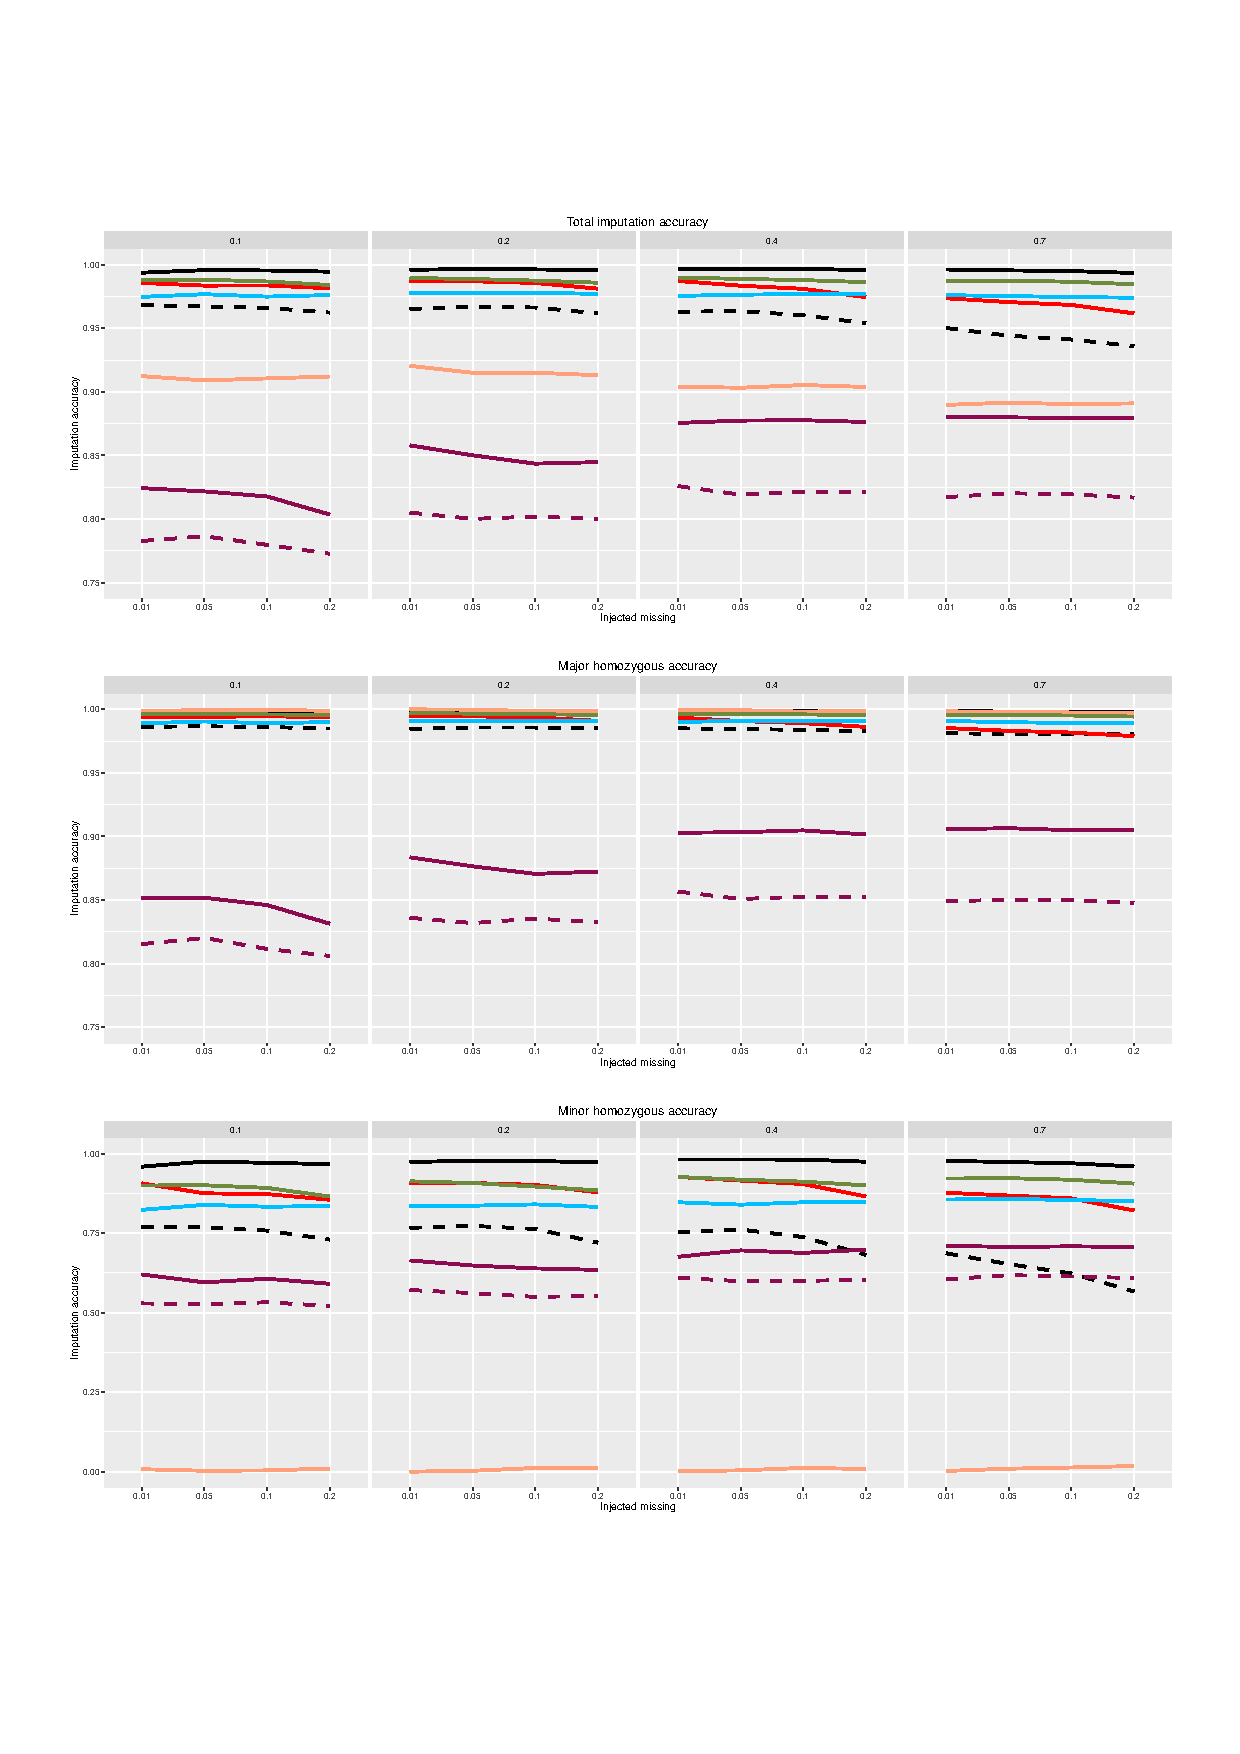
\includegraphics[width=0.95\textwidth]{figure_rice_chrom_4.pdf}\caption{
imputation accuracies overall, for the major homozygous genotype (AA) and for the minor homozygous genotype (BB) in datasets consisting of
10\%, 20\%, 40\% and 70\% allowed missing data per locus (boxes) with 1\%, 5\%, 10\% and 20\%
additional missing values artificially introduced (x-axis) for rice chromosome 4 data.
Lines colors represent the five imputation algorithms: MNI (salmon), KNNI (red), SVDI (blue), RFI (green), Beagle with ordered markers (solid black) and Beagle with unordered markers (dashed black)}\end{figure}

\begin{figure}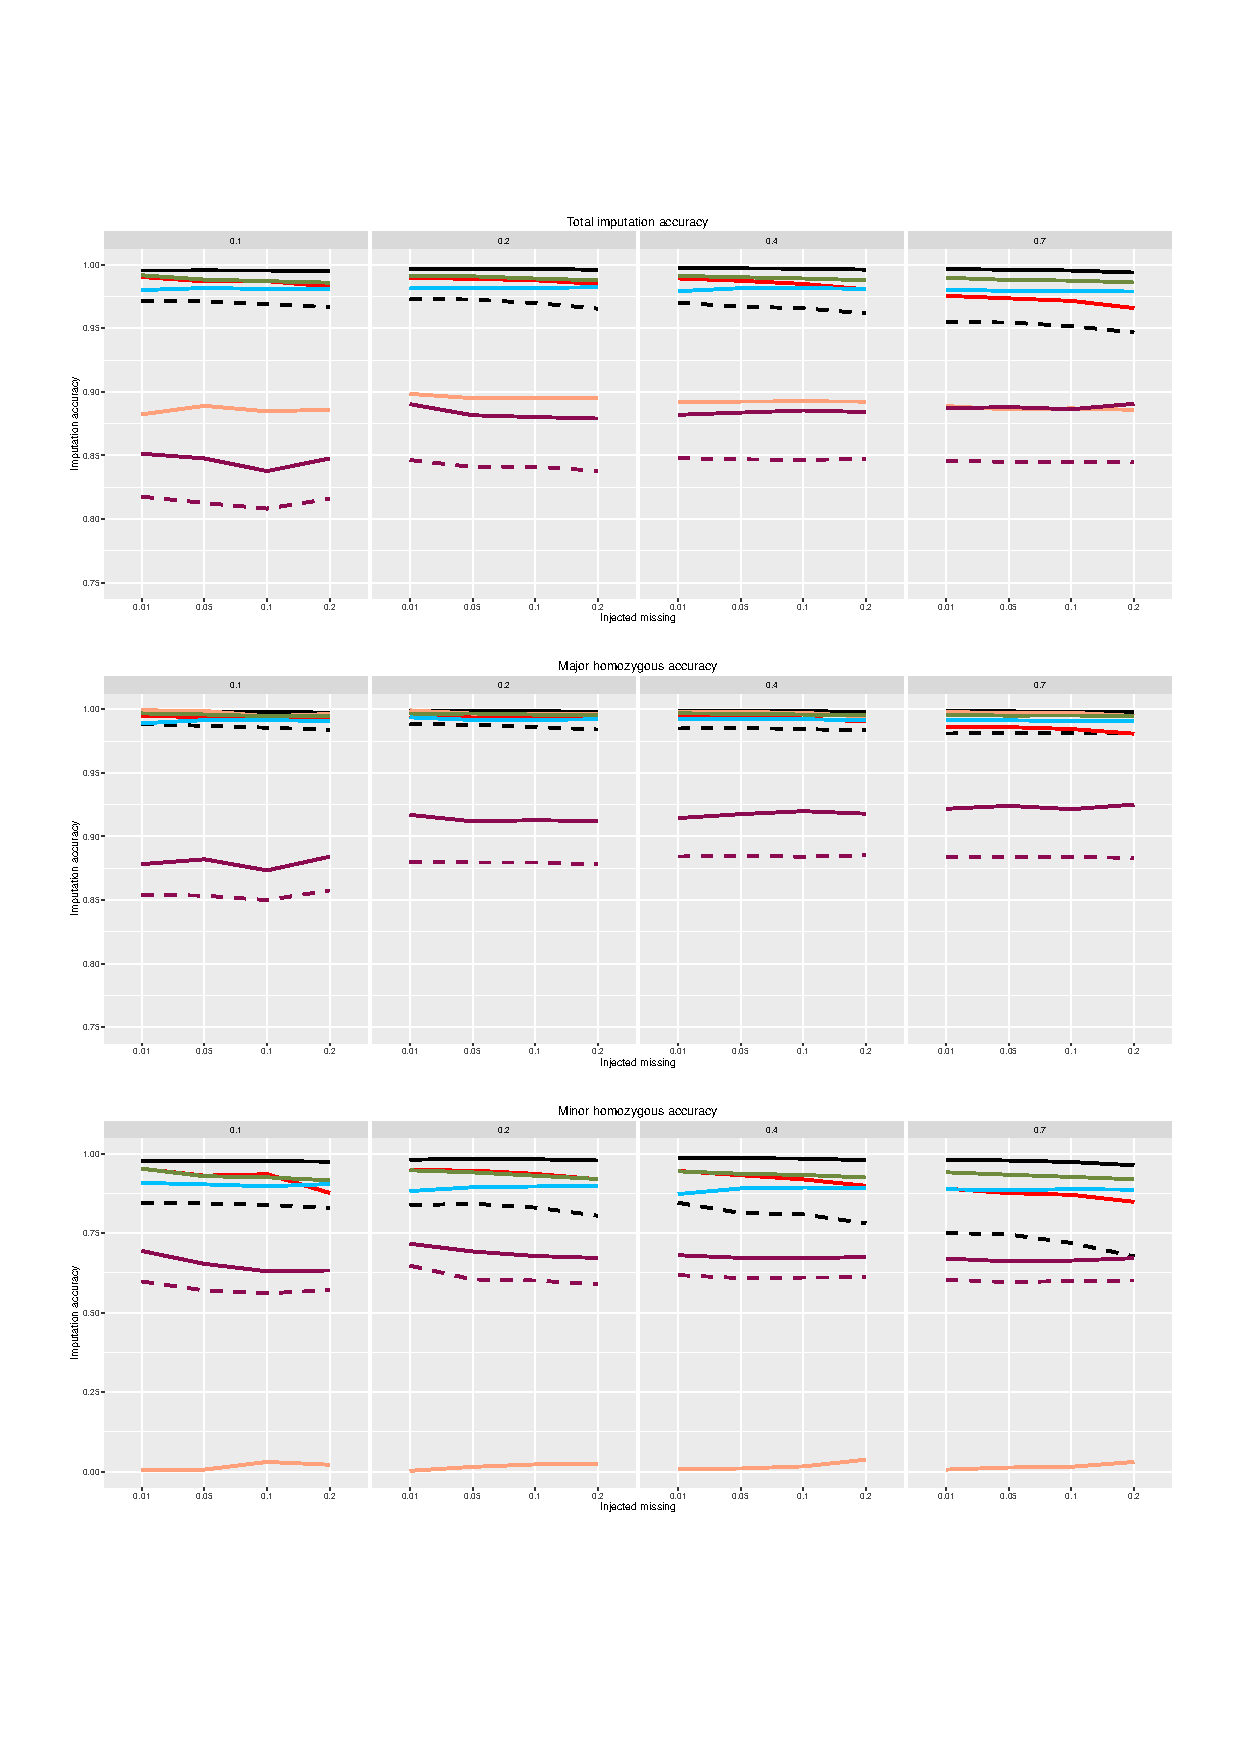
\includegraphics[width=0.95\textwidth]{figure_rice_chrom_5.pdf}\caption{
imputation accuracies overall, for the major homozygous genotype (AA) and for the minor homozygous genotype (BB) in datasets consisting of
10\%, 20\%, 40\% and 70\% allowed missing data per locus (boxes) with 1\%, 5\%, 10\% and 20\%
additional missing values artificially introduced (x-axis) for rice chromosome 5 data.
Lines colors represent the five imputation algorithms: MNI (salmon), KNNI (red), SVDI (blue), RFI (green), Beagle with ordered markers (solid black) and Beagle with unordered markers (dashed black)}\end{figure}

\begin{figure}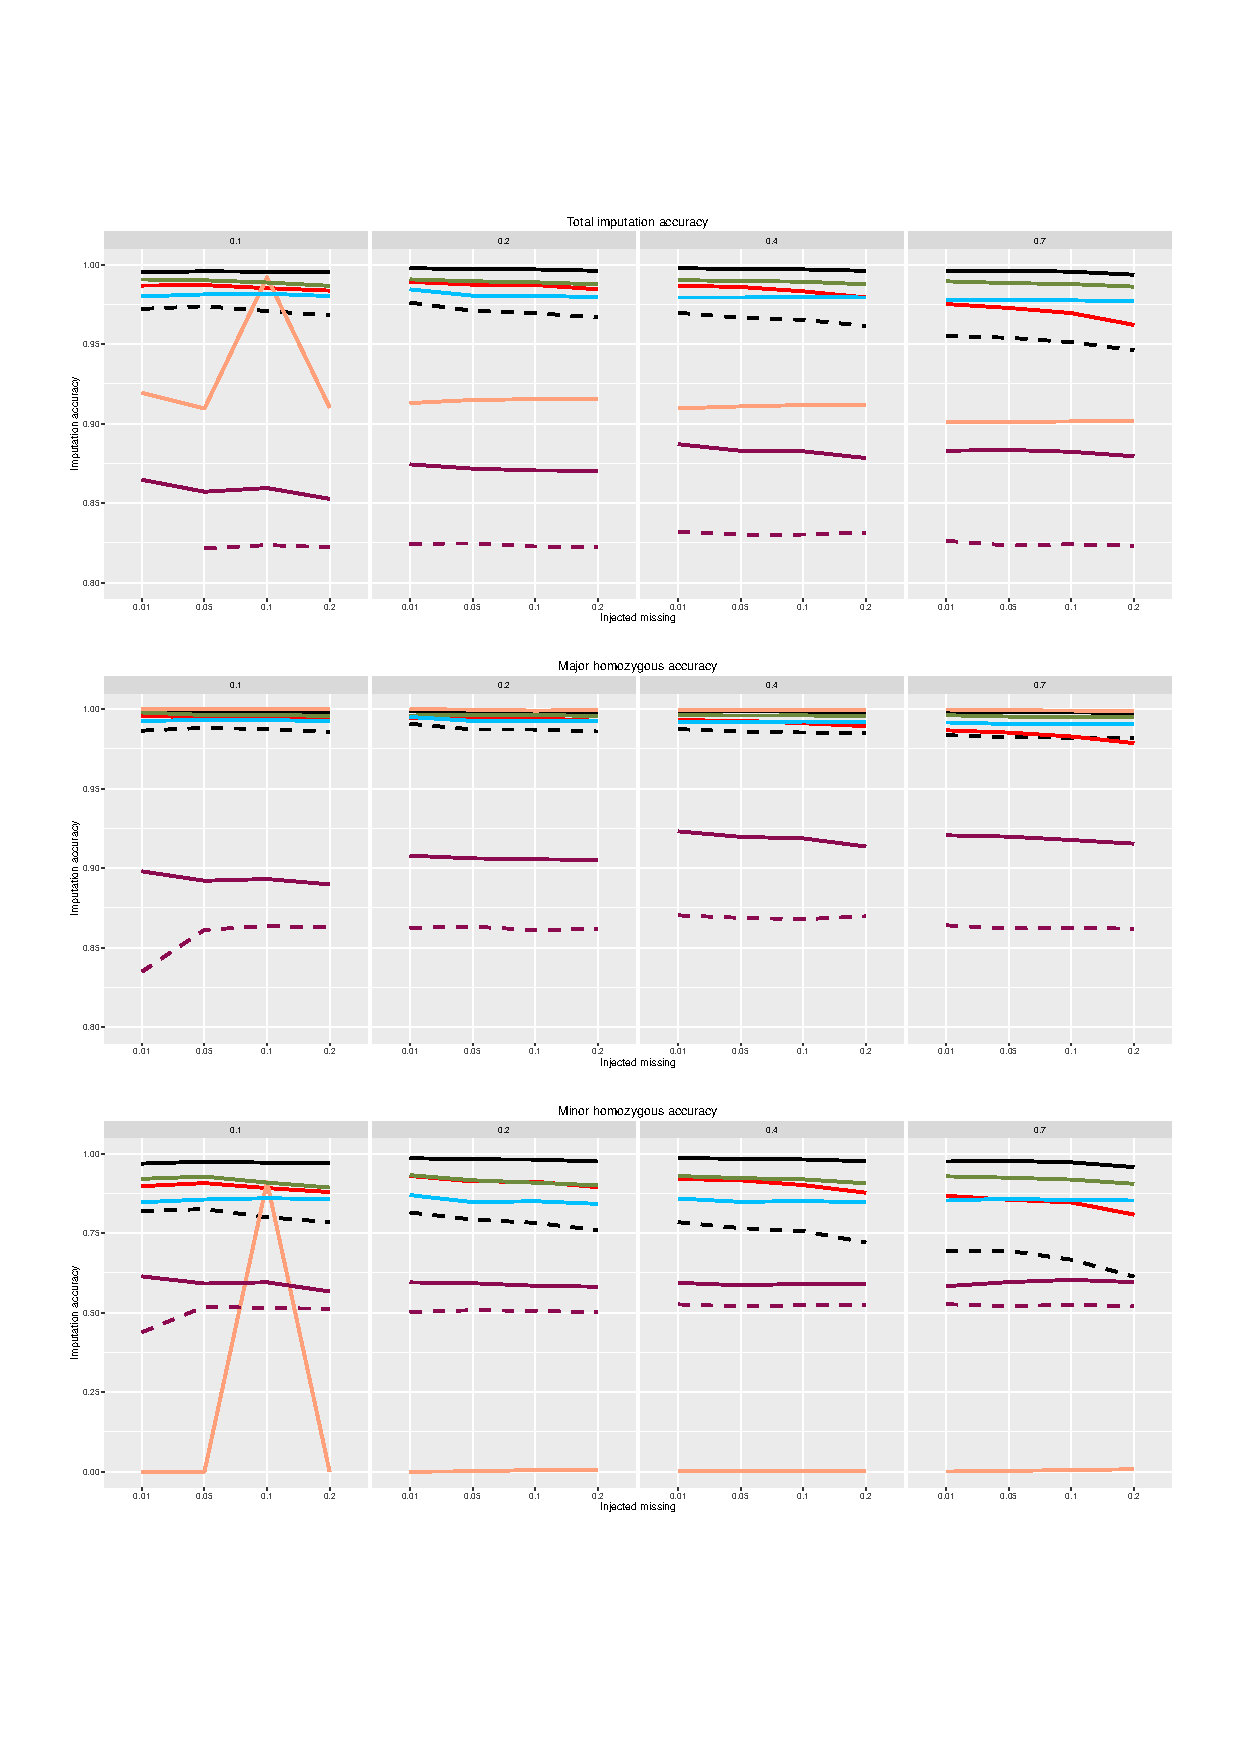
\includegraphics[width=0.95\textwidth]{figure_rice_chrom_6.pdf}\caption{
imputation accuracies overall, for the major homozygous genotype (AA) and for the minor homozygous genotype (BB) in datasets consisting of
10\%, 20\%, 40\% and 70\% allowed missing data per locus (boxes) with 1\%, 5\%, 10\% and 20\%
additional missing values artificially introduced (x-axis) for rice chromosome 6 data.
Lines colors represent the five imputation algorithms: MNI (salmon), KNNI (red), SVDI (blue), RFI (green), Beagle with ordered markers (solid black) and Beagle with unordered markers (dashed black)}\end{figure}

\begin{figure}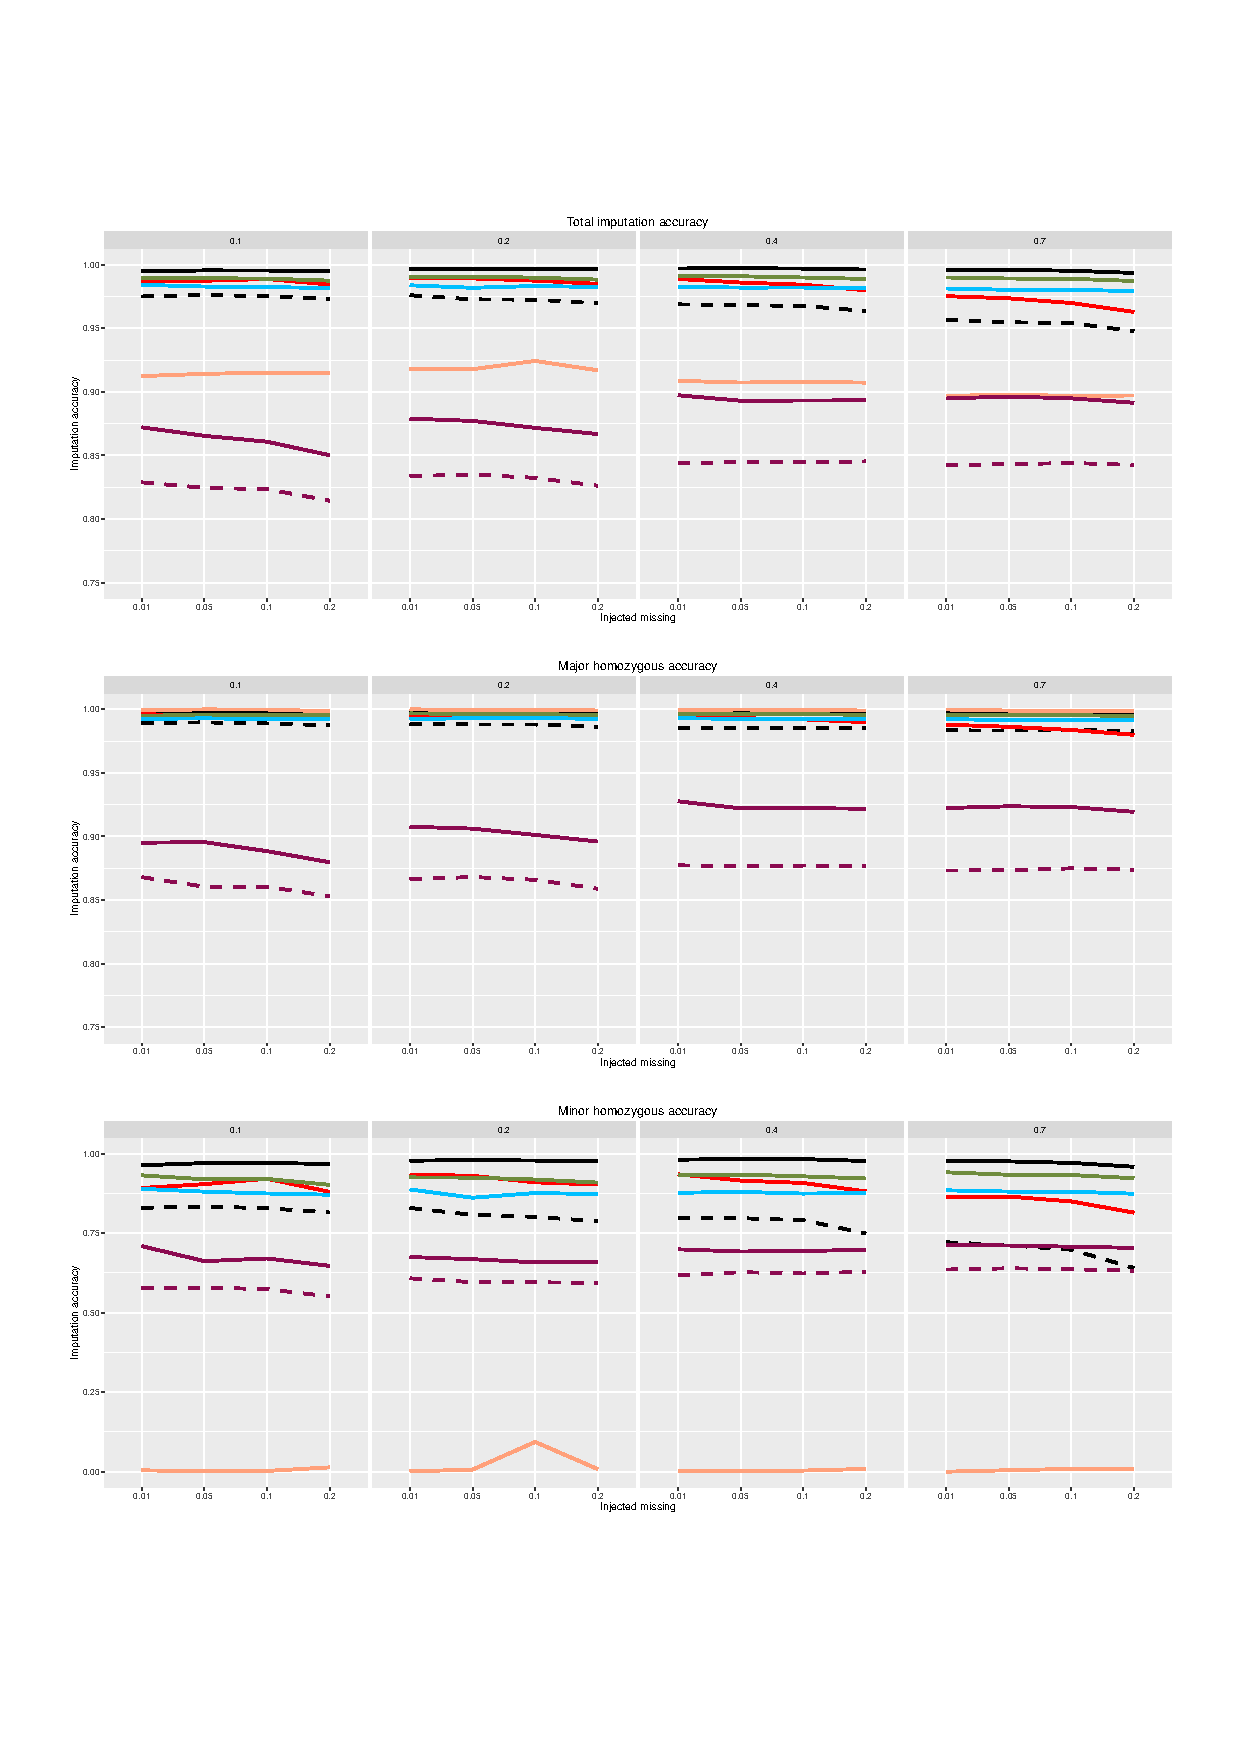
\includegraphics[width=0.95\textwidth]{figure_rice_chrom_7.pdf}\caption{
imputation accuracies overall, for the major homozygous genotype (AA) and for the minor homozygous genotype (BB) in datasets consisting of
10\%, 20\%, 40\% and 70\% allowed missing data per locus (boxes) with 1\%, 5\%, 10\% and 20\%
additional missing values artificially introduced (x-axis) for rice chromosome 7 data.
Lines colors represent the five imputation algorithms: MNI (salmon), KNNI (red), SVDI (blue), RFI (green), Beagle with ordered markers (solid black) and Beagle with unordered markers (dashed black)}\end{figure}

\begin{figure}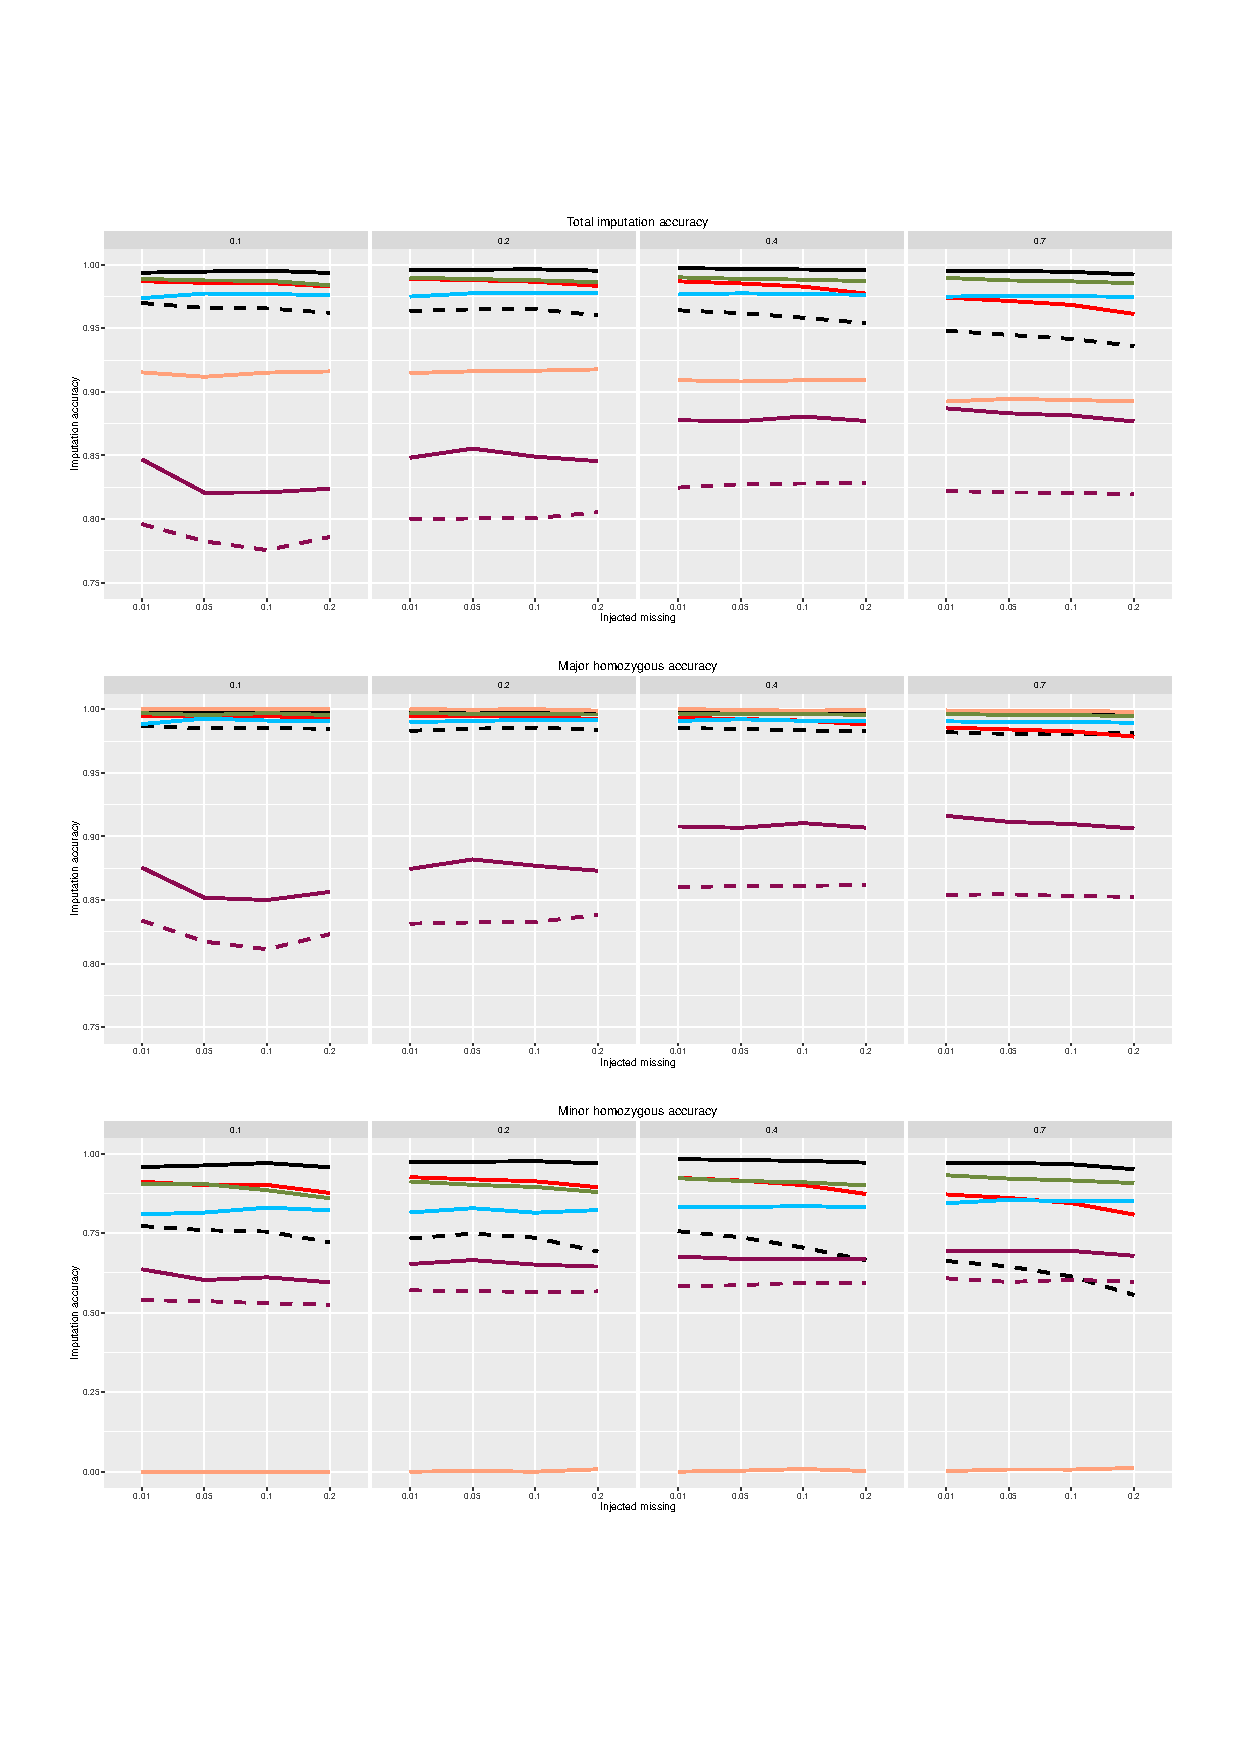
\includegraphics[width=0.95\textwidth]{figure_rice_chrom_8.pdf}\caption{
imputation accuracies overall, for the major homozygous genotype (AA) and for the minor homozygous genotype (BB) in datasets consisting of
10\%, 20\%, 40\% and 70\% allowed missing data per locus (boxes) with 1\%, 5\%, 10\% and 20\%
additional missing values artificially introduced (x-axis) for rice chromosome 8 data.
Lines colors represent the five imputation algorithms: MNI (salmon), KNNI (red), SVDI (blue), RFI (green), Beagle with ordered markers (solid black) and Beagle with unordered markers (dashed black)}\end{figure}

\begin{figure}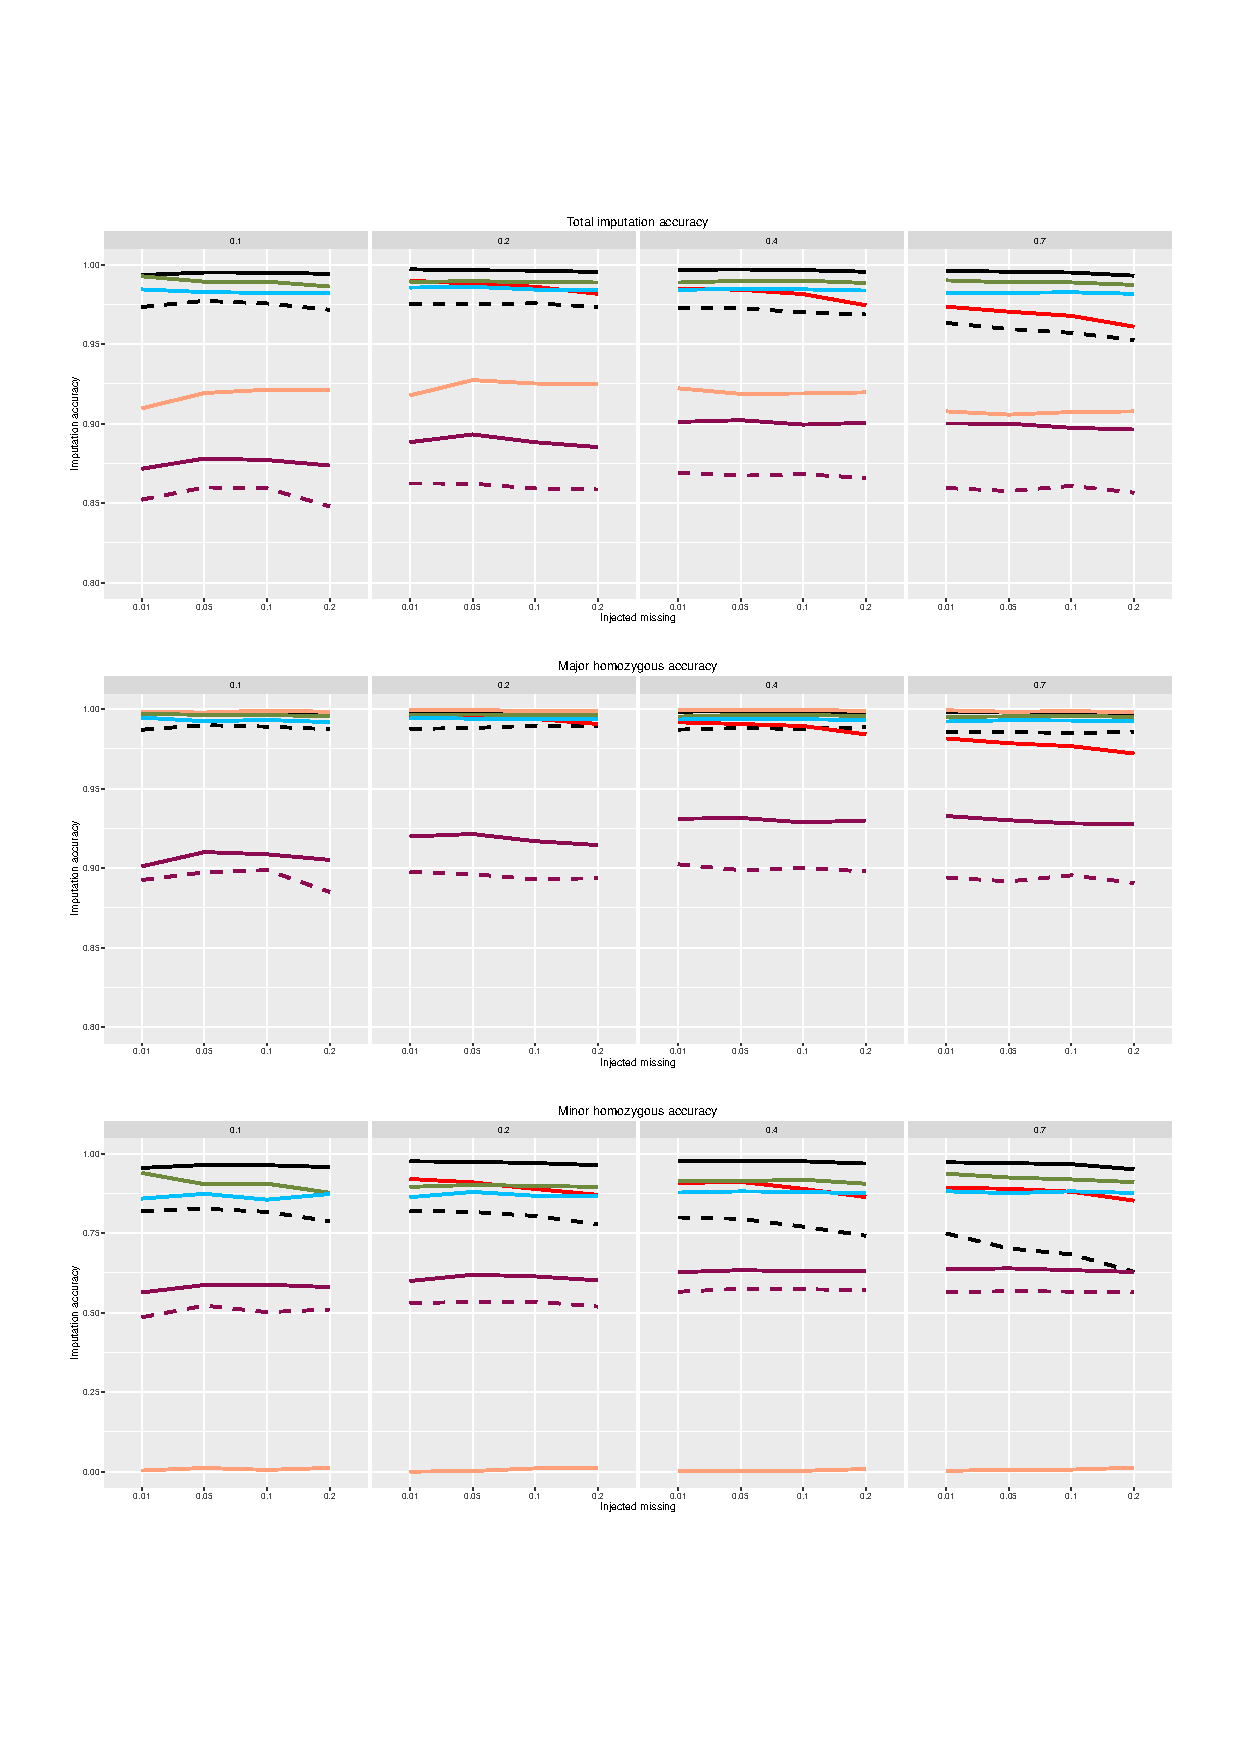
\includegraphics[width=0.95\textwidth]{figure_rice_chrom_9.pdf}\caption{
imputation accuracies overall, for the major homozygous genotype (AA) and for the minor homozygous genotype (BB) in datasets consisting of
10\%, 20\%, 40\% and 70\% allowed missing data per locus (boxes) with 1\%, 5\%, 10\% and 20\%
additional missing values artificially introduced (x-axis) for rice chromosome 9 data.
Lines colors represent the five imputation algorithms: MNI (salmon), KNNI (red), SVDI (blue), RFI (green), Beagle with ordered markers (solid black) and Beagle with unordered markers (dashed black)}\end{figure}

\begin{figure}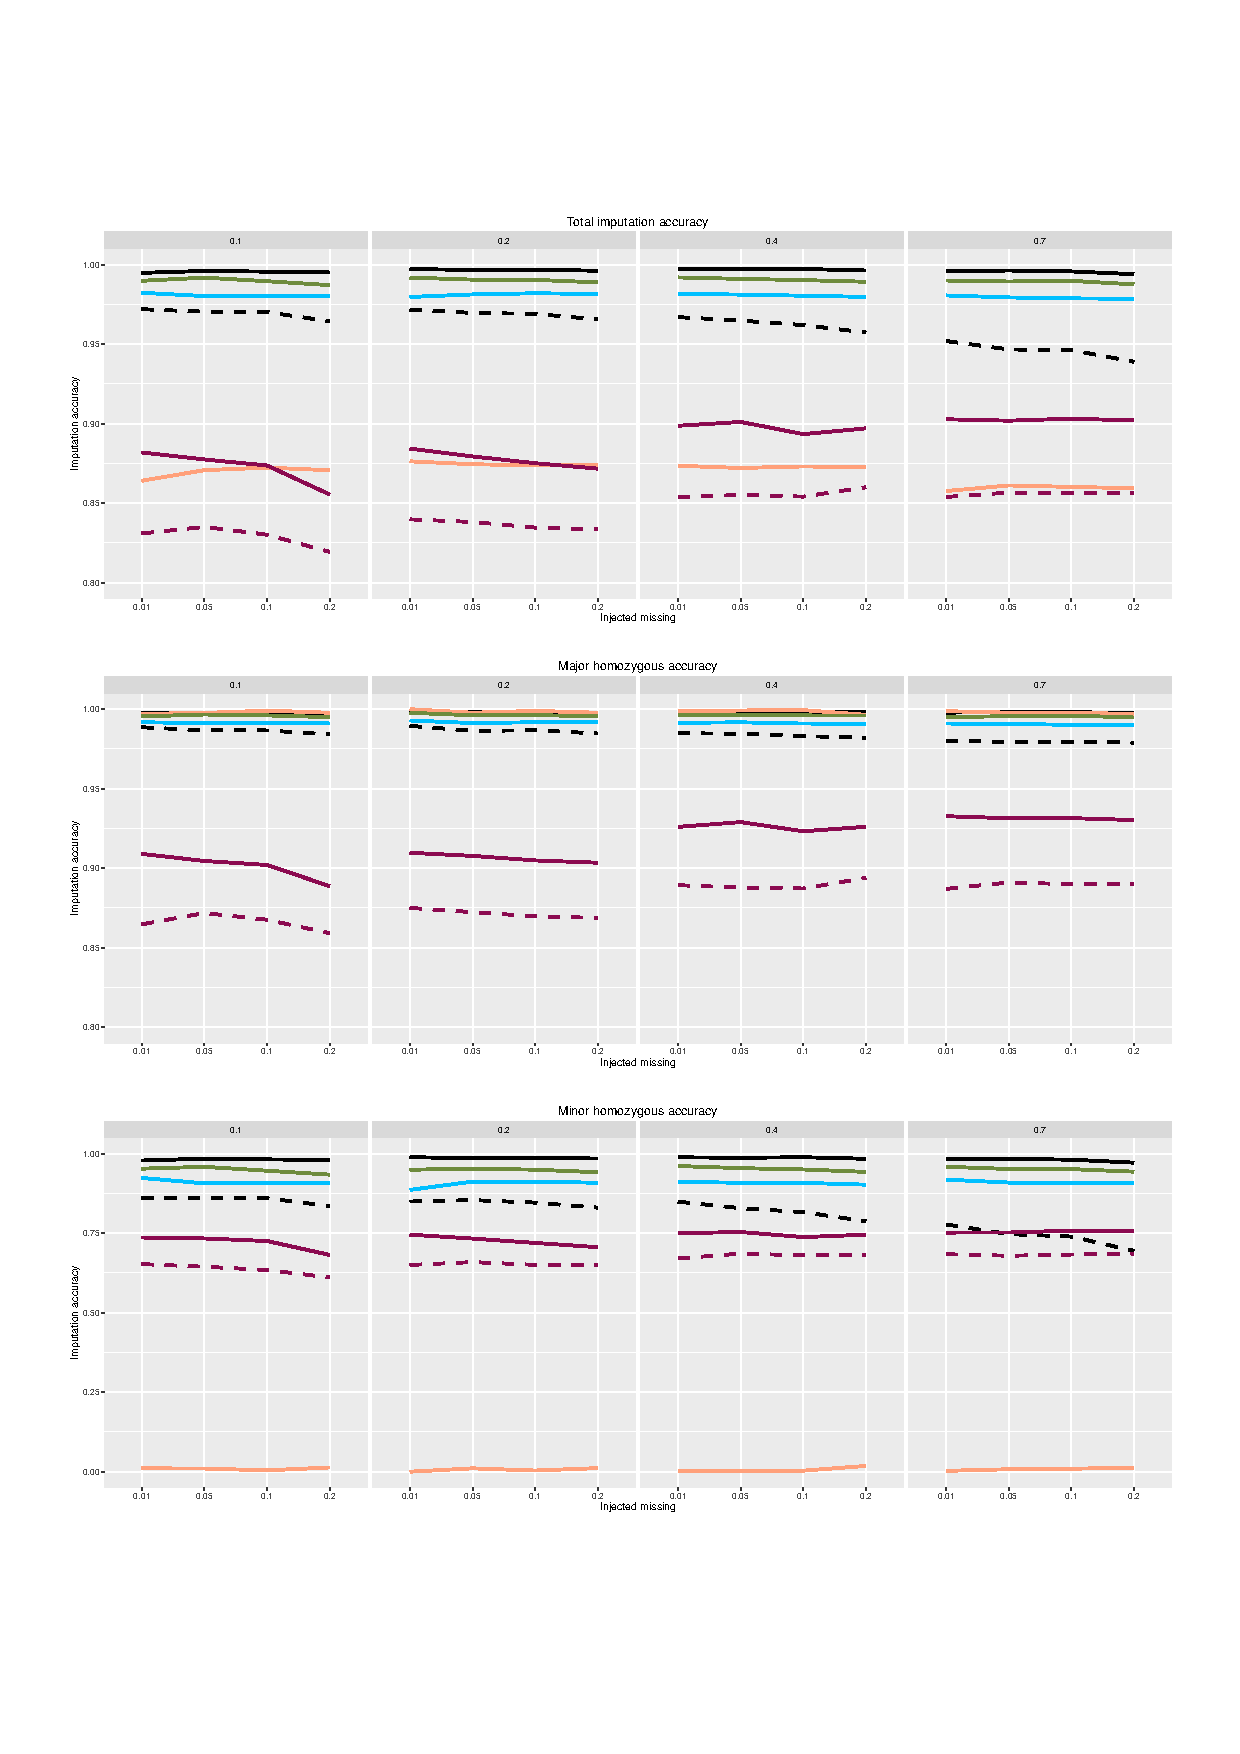
\includegraphics[width=0.95\textwidth]{figure_rice_chrom_10.pdf}\caption{
imputation accuracies overall, for the major homozygous genotype (AA) and for the minor homozygous genotype (BB) in datasets consisting of
10\%, 20\%, 40\% and 70\% allowed missing data per locus (boxes) with 1\%, 5\%, 10\% and 20\%
additional missing values artificially introduced (x-axis) for rice chromosome 10 data.
Lines colors represent the five imputation algorithms: MNI (salmon), KNNI (red), SVDI (blue), RFI (green), Beagle with ordered markers (solid black) and Beagle with unordered markers (dashed black)}\end{figure}
\begin{figure}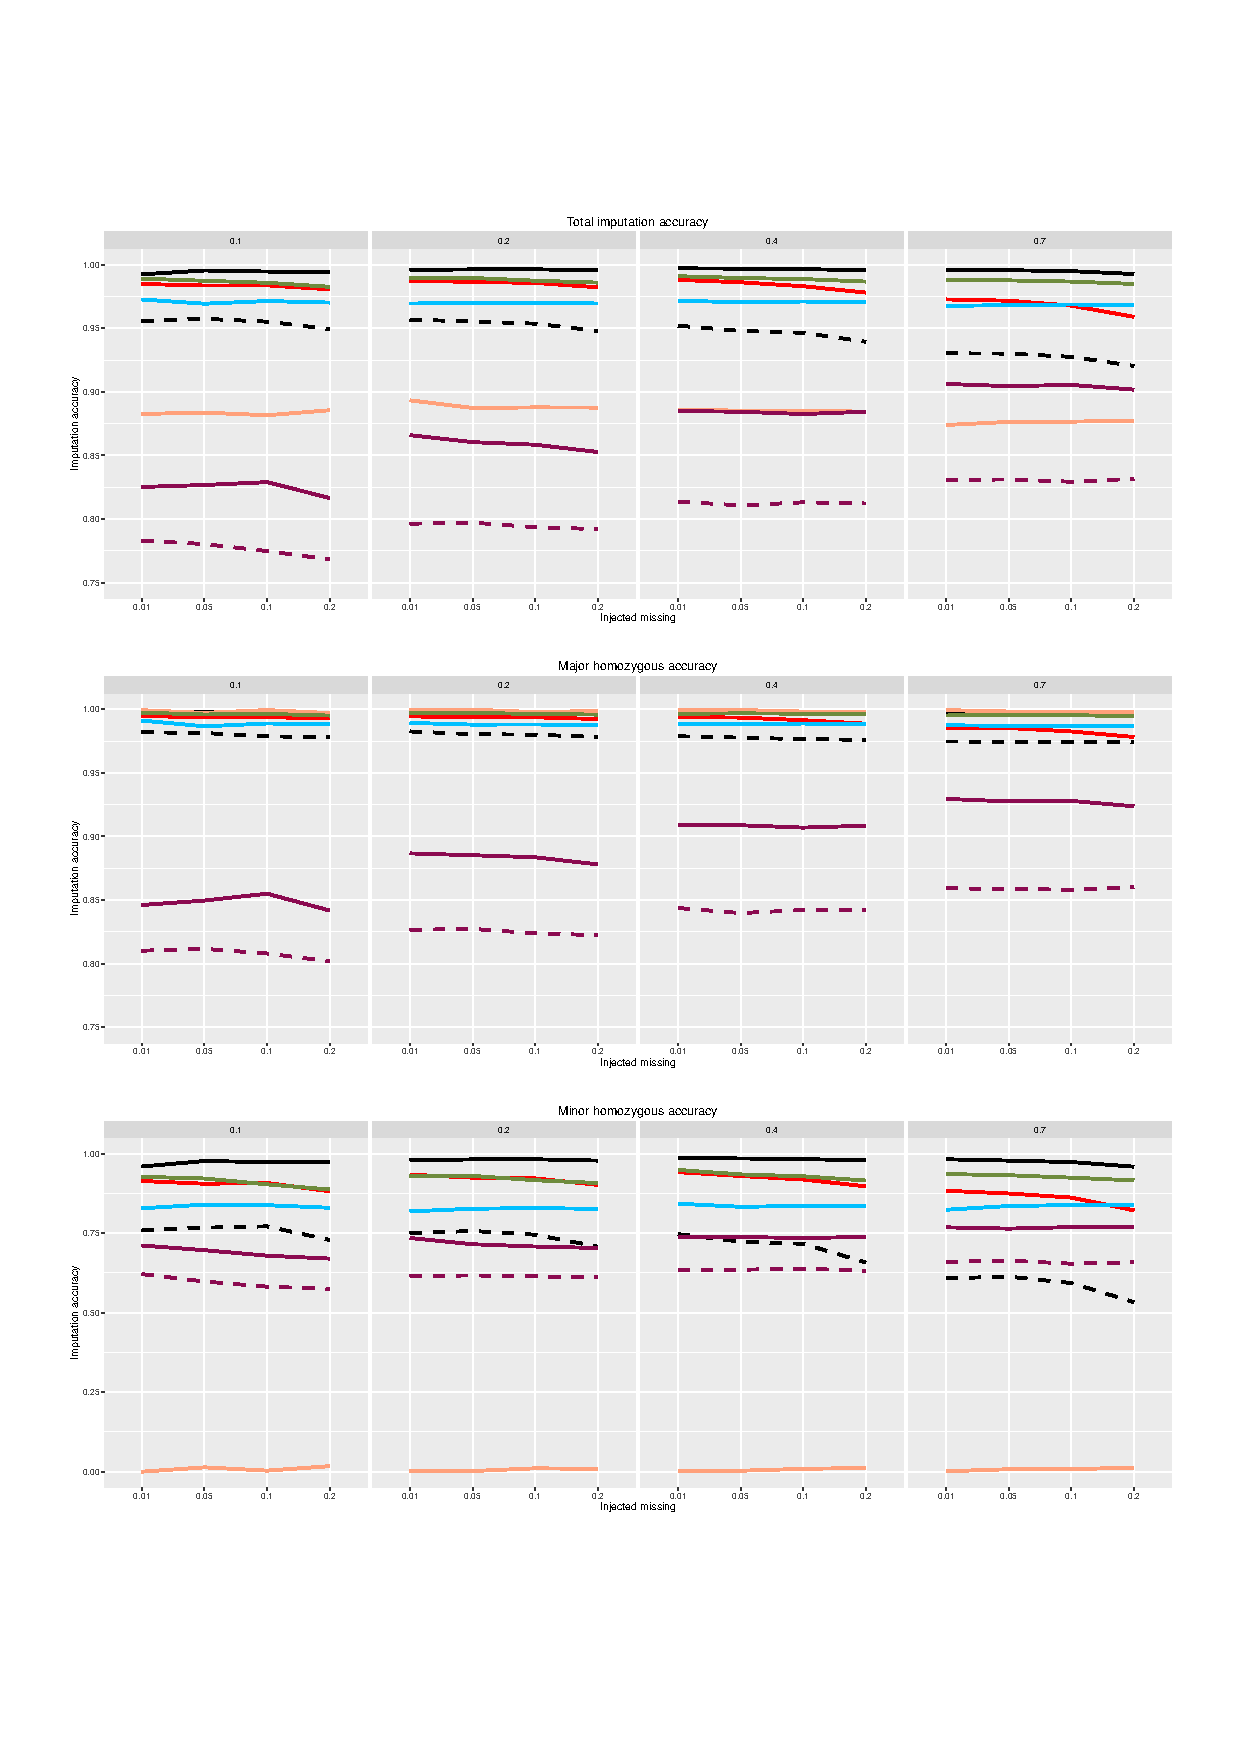
\includegraphics[width=0.95\textwidth]{figure_rice_chrom_11.pdf}\caption{
imputation accuracies overall, for the major homozygous genotype (AA) and for the minor homozygous genotype (BB) in datasets consisting of
10\%, 20\%, 40\% and 70\% allowed missing data per locus (boxes) with 1\%, 5\%, 10\% and 20\%
additional missing values artificially introduced (x-axis) for rice chromosome 11 data.
Lines colors represent the five imputation algorithms: MNI (salmon), KNNI (red), SVDI (blue), RFI (green), Beagle with ordered markers (solid black) and Beagle with unordered markers (dashed black)}\end{figure}

\begin{figure}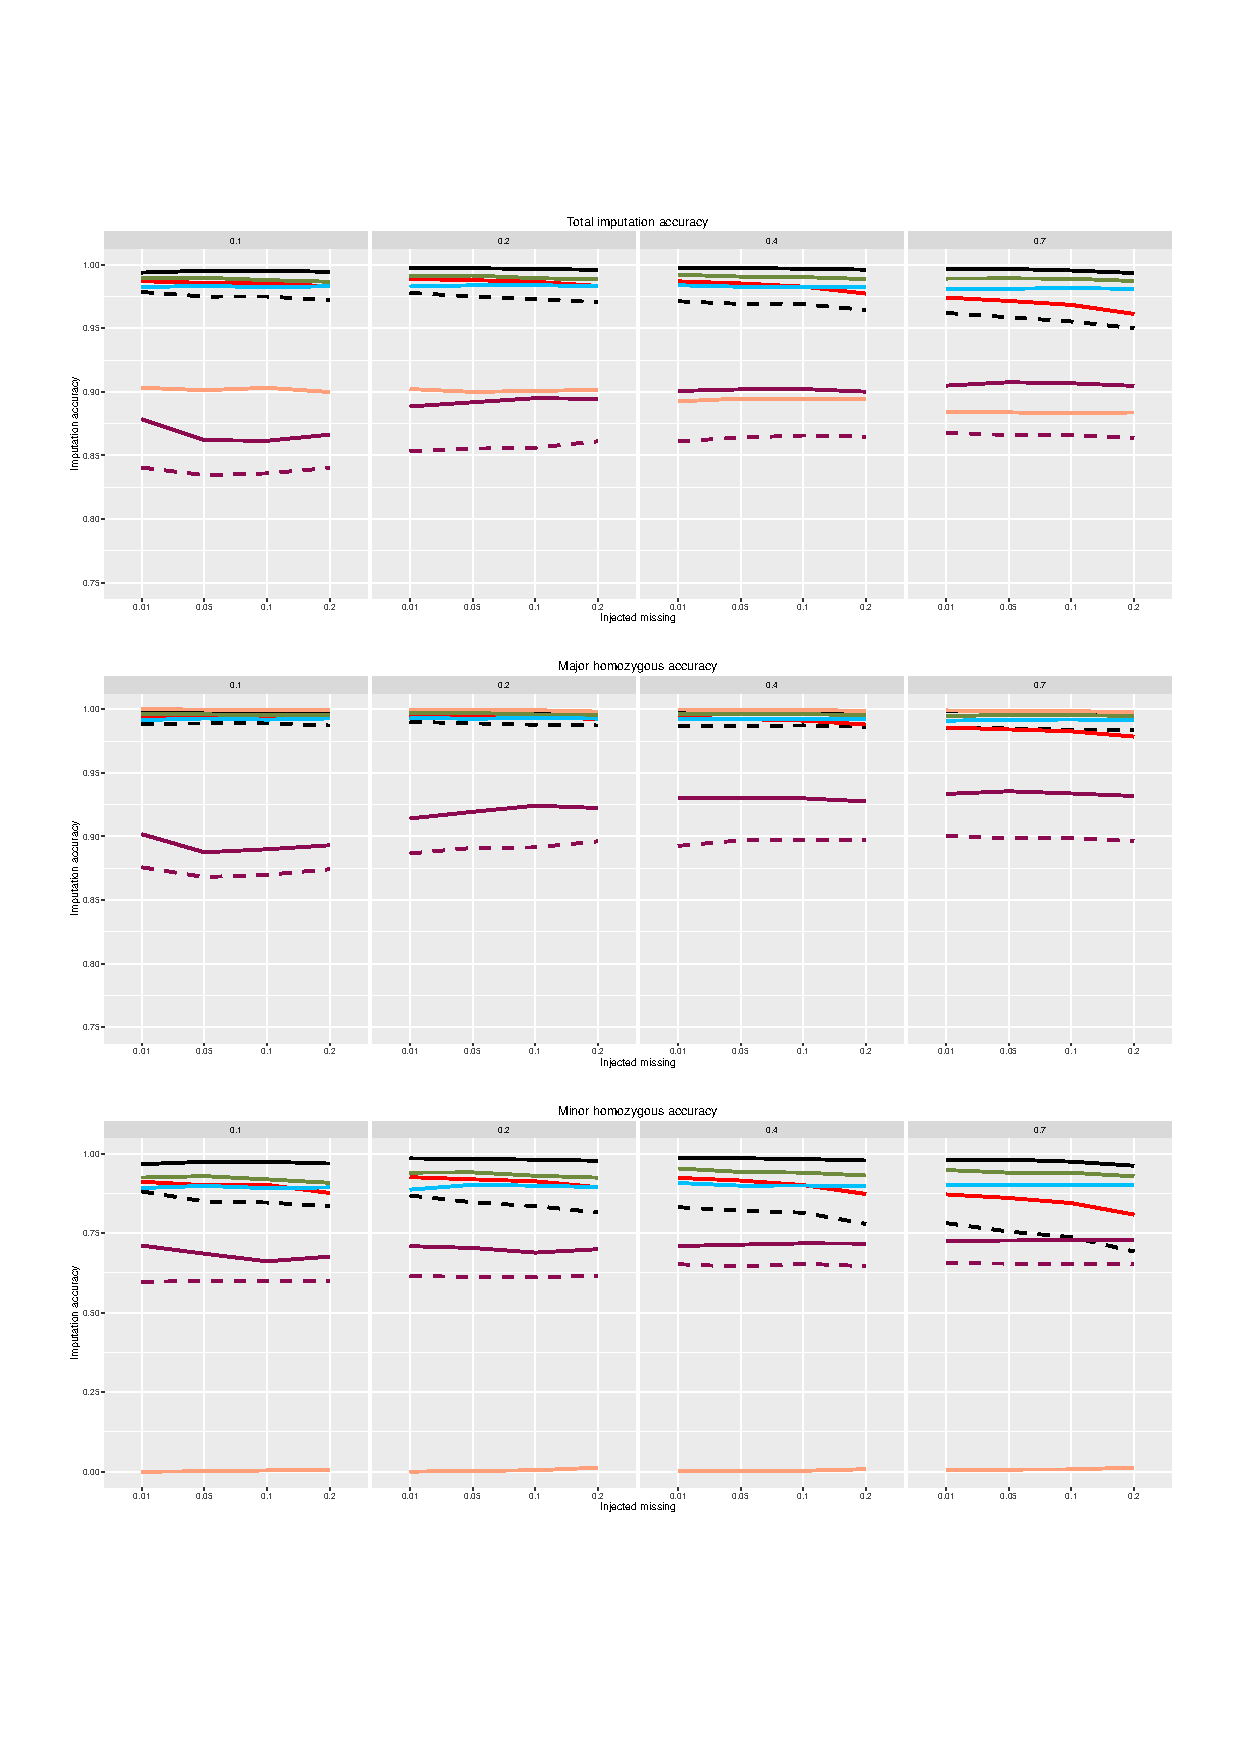
\includegraphics[width=0.95\textwidth]{figure_rice_chrom_12.pdf}\caption{
imputation accuracies overall, for the major homozygous genotype (AA) and for the minor homozygous genotype (BB) in datasets consisting of
10\%, 20\%, 40\% and 70\% allowed missing data per locus (boxes) with 1\%, 5\%, 10\% and 20\%
additional missing values artificially introduced (x-axis) for rice chromosome 12 data.
Lines colors represent the five imputation algorithms: MNI (salmon), KNNI (red), SVDI (blue), RFI (green), Beagle with ordered markers (solid black) and Beagle with unordered markers (dashed black)}\end{figure}

\begin{figure}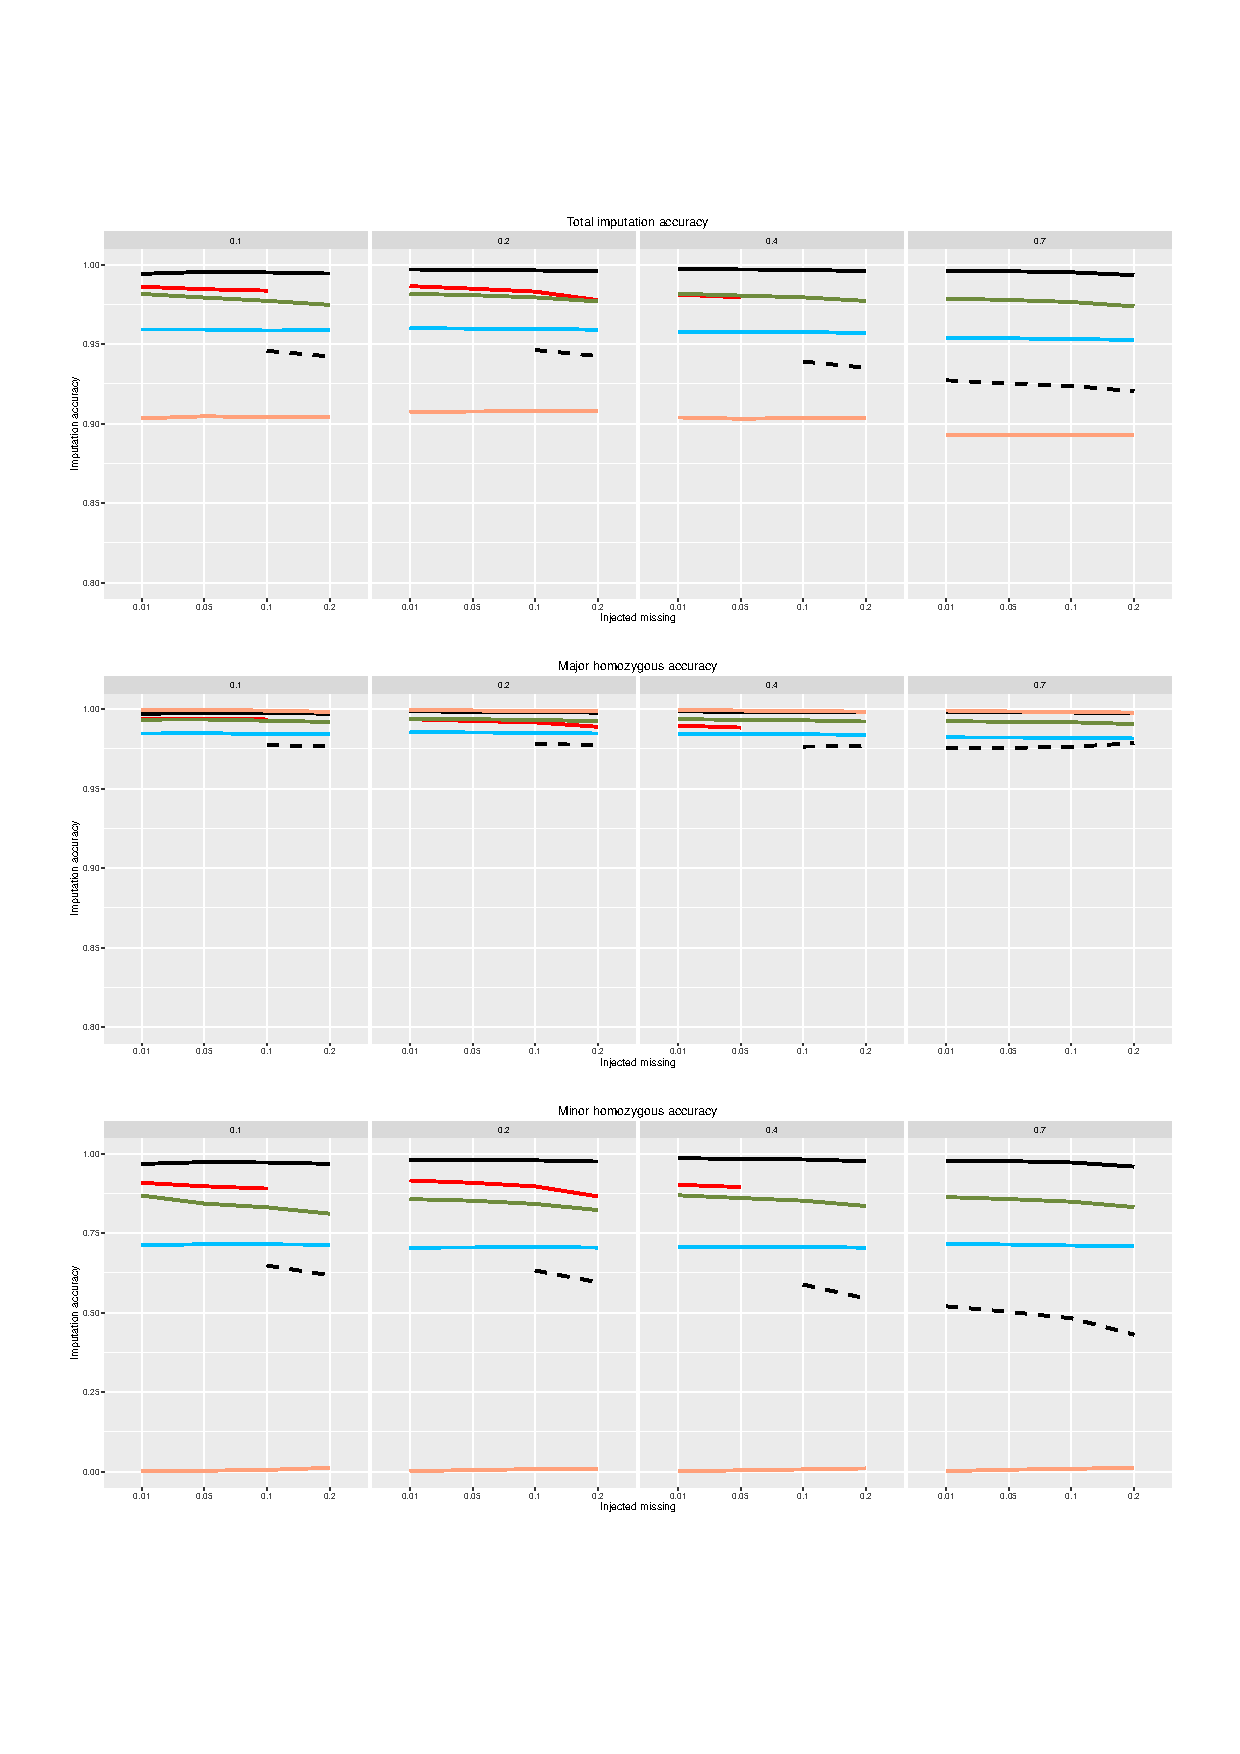
\includegraphics[width=0.95\textwidth]{figure_rice.pdf}\caption{
imputation accuracies overall, for the major homozygous genotype (AA) and for the minor homozygous genotype (BB) in datasets consisting of
10\%, 20\%, 40\% and 70\% allowed missing data per locus (boxes) with 1\%, 5\%, 10\% and 20\%
additional missing values artificially introduced (x-axis) for whole rice data set.
Lines colors represent the five imputation algorithms: MNI (salmon), KNNI (red), SVDI (blue), RFI (green), Beagle with ordered markers (solid black) and Beagle with unordered markers (dashed black)}\end{figure}













 




